\definecolor{green}{cmyk}{0,0.25,0.5,0}
\definecolor{orange}{cmyk}{0,0.25,0.5,0}
\newcommand{\weblong}[2]{\href{#1}{#2}} % definition of long hyperreferences
\newcommand {\key}[1]{\textbf{\ttfamily{#1}}} % definition of key
\newcommand {\button}[1]{\textbf{\sffamily{#1}}} % definition of GUI button
\newcommand {\command}[1]{{\ttfamily{#1}}} % definition of console command
\newcommand {\excl}[1]{
    \begin{tabular}{r p{0.75\textwidth}}
    \hspace*{5mm}\LARGE{\textcolor{green}{$!$
    %\ArrowBoldDownRight
}} & #1\\
\end{tabular}
}
\newcommand {\photo}[3]
{\begin{center}
  \includegraphics[width=0.5\textwidth]{img/#3}
\end{center}}

%%%%%%%%%%%%%%%%%%%%%%%%%%%%%%%%%%%%%%%%%%%%%%%%%%%%%%%%%%%%%%%%%%%%
\ifchinese
\chapter{{\\}基础飞行模拟教程}
\fi
\iffalse
\IfLanguageName{english}{
\chapter{A Basic Flight Simulator Tutorial}
}{}
\fi
\IfLanguageName{french}{
\chapter{Un tutoriel de base de simulation de vol}
}{}
\label{basic}
%%%%%%%%%%%%%%%%%%%%%%%%%%%%%%%%%%%%%%%%%%%%%%%%%%%%%%%%%%%%%%%%%%%%

\ifchinese
\section{序言}
\fi
\iffalse
\IfLanguageName{english}{
\section{Foreword}
}{}
\fi
\IfLanguageName{french}{
\section{Pr\'{e}ambule}
}{}
\label{sec:Foreword}

\ifchinese
航空业充满了各种极端:
\begin{itemize}
\item 飞机非常脆弱却以高速飞行。然而却是最安全的交通工具。
\item 飞行员需要紧跟各种规则和程序。然而飞机却是自由的象征。
\item 只需要很少的一些训练,飞小型飞机是很容易的。然而一旦发生问题,需要在数秒内解决。
\item 很多飞行教程都以幽默的口吻来写,然而若飞行时不够严肃,会让你快速坠地。
\end{itemize}
\fi
\iffalse
\IfLanguageName{english}{
Aviation is about extremes:
\begin{itemize}
    \item An airplane is quite fragile and flies at high speeds.
  Yet it is one of the safest forms of transport.
    \item Pilots must constantly follow rules and procedures.
  Yet an airplane is a symbol of freedom.
    \item With a little training, flight a small aircraft is easy.
  Yet if a problem occurs, you must be able to resolve it in a few seconds.
    \item Many flight tutorials are written with a lot of humor.
  Yet not taking flying seriously will bring you down to earth prematurely.
\end{itemize}
}{}\fi

\IfLanguageName{french}{
L'aviation est faite d'extr\^{e}mes :

\begin{itemize}
    \item Un a\'{e}ronef est assez fragile et vole \`{a} des vitesses \'{e}lev\'{e}es.
  Cependant, c'est l'un des moyens de transports les plus s\^{u}rs.
    \item Les pilotes doivent constamment suivre des r\`{e}gles et des proc\'{e}dures.
  Cependant, un a\'{e}ronef est un symbole de libert\'{e}.
    \item Avec un peu d'entra\^{i}nement, voler un petit a\'{e}ronef est simple.
  Cependant, si un probl\`{e}me survient, vous devez \^{e}tre capable de le r\'{e}soudre en quelques secondes.
    \item De nombreux tutoriels de vols sont \'{e}crits avec beaucoup d'humour.
  Cepedant, ne pas prendre le vol au s\'{e}rieux vous rem\`{e}nera sur le plancher des vaches de mani\`{e}re pr\'{e}matur\'{e}e.
\end{itemize}
}{}

\ifchinese
此教程使用的飞行器是\weblong{http://en.wikipedia.org/wiki/Cessna_172} {塞斯纳 172P}\footnote{塞斯纳 172 对中国人来说并不陌生,在上世纪八十年代风靡全国的日本电影《追捕》中,杜秋冬人(高仓健饰)就是驾驶塞斯纳 172R 飞机从北海道飞回本州的。——译者注} 型。此机型已被用于很多真实飞行学校中,并且是一款非常好飞的机型。
\fi
\iffalse
\IfLanguageName{english}{
The aircraft used in this tutorial is the
\weblong{http://en.wikipedia.org/wiki/Cessna_172} {Cessna 172p}. This is the
aircraft used in many real life flight schools and a great airplane to fly.
}{}
\fi

\IfLanguageName{french}{
L'a\'{e}ronef utilis\'{e} dans ce tutoriel est le
\weblong{http://en.wikipedia.org/wiki/Cessna_172} {Cessna 172p}. Il s'agit de l'avion
utilis\'{e} dans de nombreuses v\'{e}ritables \'{e}coles de pilotage et c'est un avions tr\`{e}s agr\'{e}able en vol.
}{}

\begin{center}
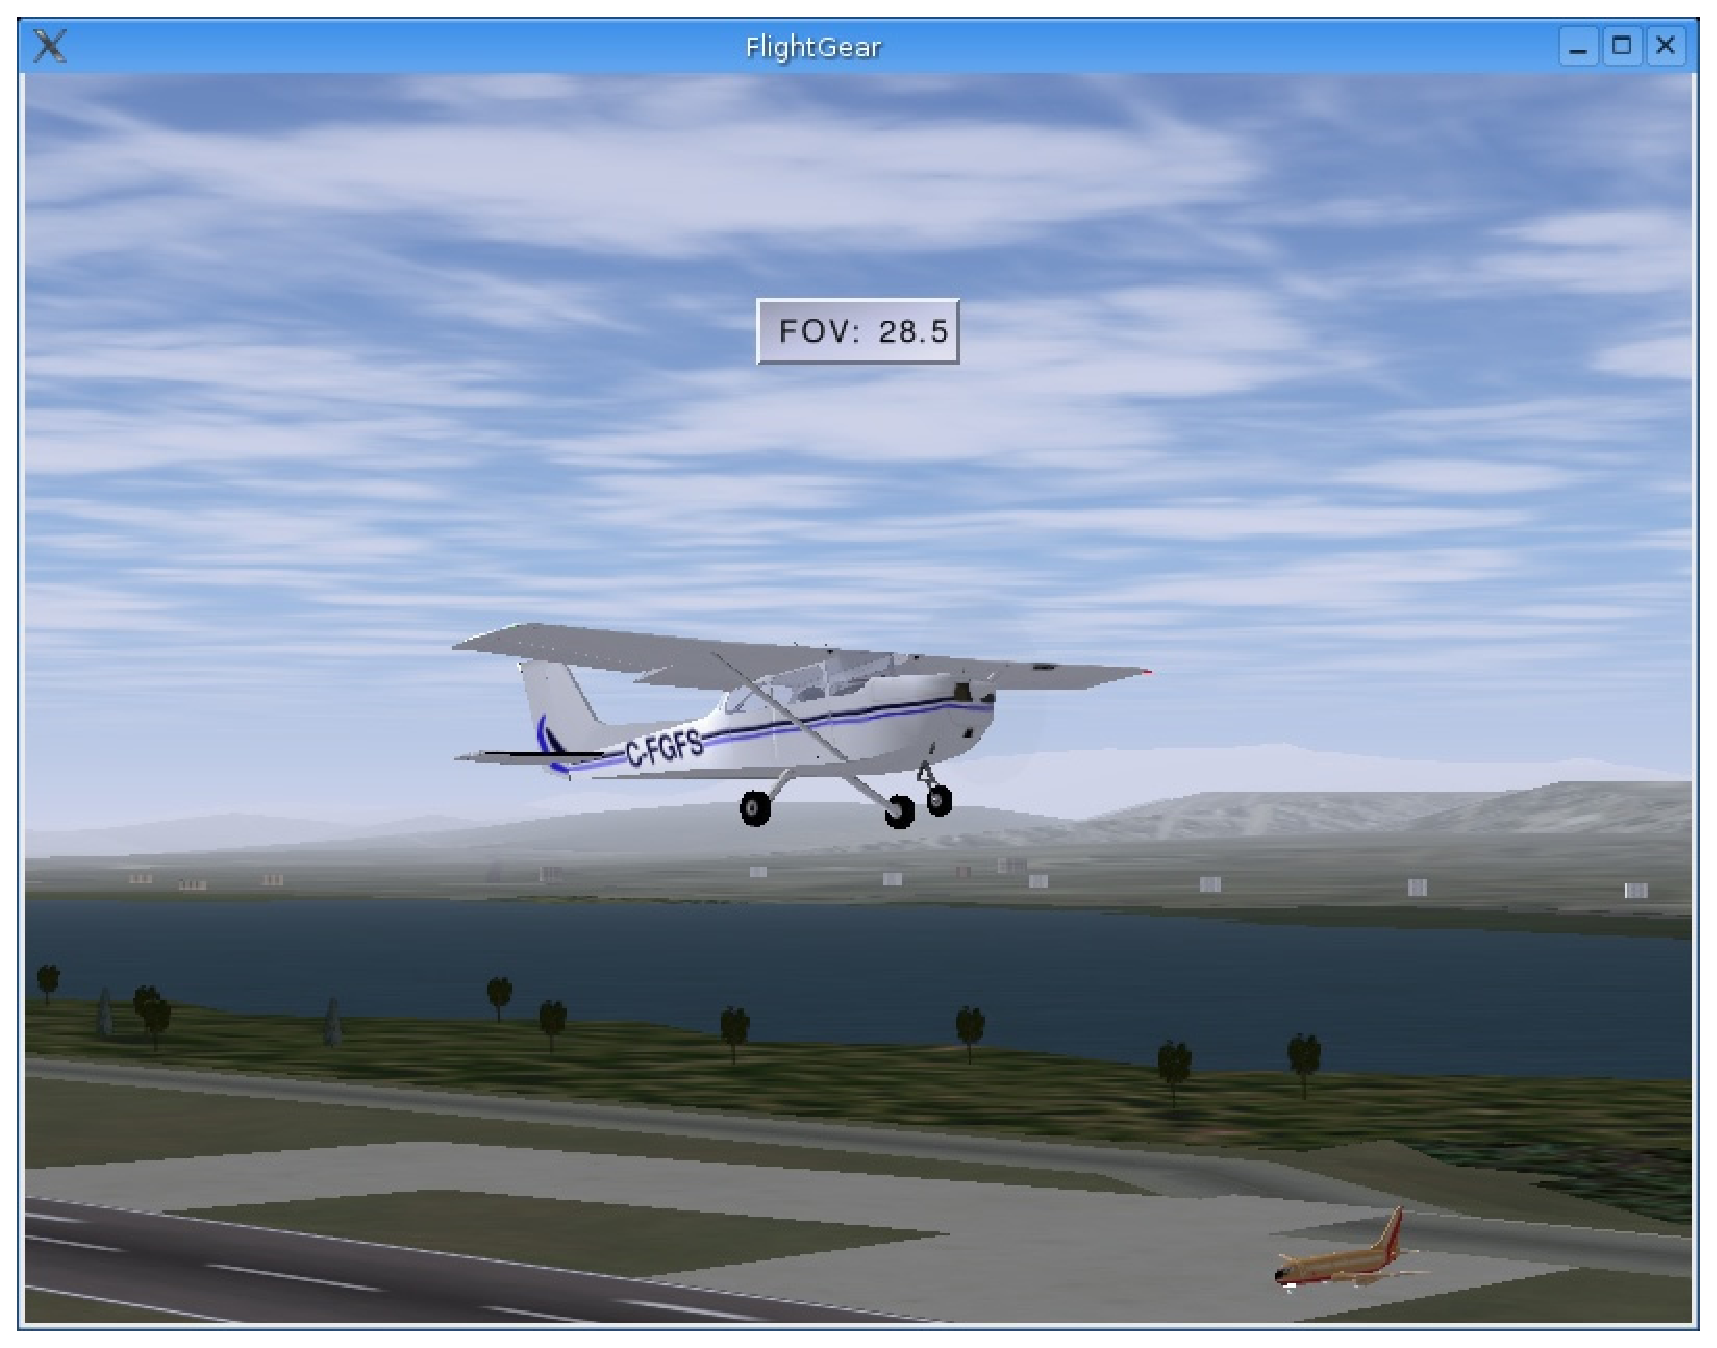
\includegraphics[width=0.5\textwidth]{img/tut_1}
\end{center}

\ifchinese
下面的这些文章可以作为此教程的补充,并回答了很多你阅读中的一些问题。特别是第一篇介绍了飞机的主要部件和控制:
\fi
\iffalse
\IfLanguageName{english}{
The following articles complement this tutorial and will answer most questions
that may arise as you read through. The first one in particular is a good
introduction to the airplane's main components and controls:
}{}
\fi
\IfLanguageName{french}{
Les articles suivants compl\`{e}tent ce tutoriel et r\'{e}pondront \`{a} la plupart des questions qui pourraient
survenir lors de votre lecture. Le premier, en particulier, est une bonne
introduction aux principaux composants et contr\^{o}les de l'a\'{e}ronef :
}{}

\begin{itemize}
    \item \weblong{https://www.gleim.com/aviation/learn-to-fly/}    {https://www.gleim.com/aviation/learn-to-fly/}
    \item \weblong{http://www.pilotfriend.com/training/flight\_training/aero/principa.htm}    {http://www.pilotfriend.com/training/flight\_training/aero/principa.htm}
    \item \web{http://en.wikipedia.org/wiki/Aircraft}
    \item \web{http://en.wikipedia.org/wiki/Flight\_controls}
    \item \web{http://en.wikipedia.org/wiki/Airplane\_flight\_mechanics}
    \item \web{http://en.wikipedia.org/wiki/Aircraft\_engine\_controls}
    \item \web{http://www.firstflight.com/flt1.html}
    \item \web{http://flightsims.ig-wilson.com/index.php?f16land}
    \item \web{http://www.navfltsm.addr.com/}
\end{itemize}

\ifchinese
此教程基于我本人的知识,然而不可避免的可能会有一些错误。对此我非常抱歉。
\fi
\iffalse
\IfLanguageName{english}{
This tutorial is accurate to the best of my knowledge, but will inevitably
contain some mistakes. I apologize in advance for these.
}{}
\fi
\IfLanguageName{french}{
Ce tutoriel est pr\'{e}cis dans les limites de mes meilleures connaissances, mais il contiendra in\'{e}vitablement
quelques erreurs. Je m'excuse par avance pour celles-ci.
}{}

\ifchinese
\section{启动}
\fi
\iffalse
\IfLanguageName{english}{
\section{Starting Up}
}{}
\fi
\IfLanguageName{french}{
\section{D\'{e}marrer}
}{}
\ifchinese
根据你的平台和发行版的不同,有很多种方式来启动 \FlightGear{}。
\fi
\iffalse
\fi
\IfLanguageName{english}{
There are a number of different ways to start \FlightGear{} based on your
platform and the distribution you are using.
}{}
\IfLanguageName{french}{
Il existe diff\'{e}rentes mani\`{e}res de d\'{e}marrer \FlightGear{} en fonction de la
plate-forme et de la distribution que vous utilisez.
}{}

\subsection{MS Windows}
\ifchinese
在微软 Windows 系统中,\FlightGear{} 有一个图形化的向导,让你可以选择飞行器和起始位置。首先如下图所示选择 Cessna 172p 飞机。为了能够适应此教程,不要选择 2D 仪表板的版本(你也许会发现 2D 仪表板更适宜教学)。点击\button{下一步}按钮来选择机场。
\fi
\iffalse
\IfLanguageName{english}{
On MS Windows, \FlightGear{} has a GUI Wizard in which you can choose your
aircraft and starting postion. First choose the Cessna 172p airplane as shown
below. To match this tutorial do not choose the 2D panel version.
(You may however find in the future that the 2D version is more appropriate
for training). Click the \button{Next} button to choose your airport.
}{}
\fi
\IfLanguageName{french}{
Sur MS Windows, \FlightGear{} dispose d'un assistant en mode graphique dans
lequel vous pouvez choisir votre a\'{e}ronef et votre position de d\'{e}marrage.
Choisissez d'abord l'a\'{e}ronef Cessna 172p comme montr\'{e} ci-dessous.
Pour correspondre \`{a} ce tutoriel, ne choisissez pas la version avec panneau 2D.
(Vous pourriez cependant trouver dans le futur que la version 2D est plus
appropri\'{e}e pour l'entra\^{i}nement. Cliquez sur le bouton \button{Suivant}
pour choisir votre a\'{e}roport.
}{}

\begin{center}
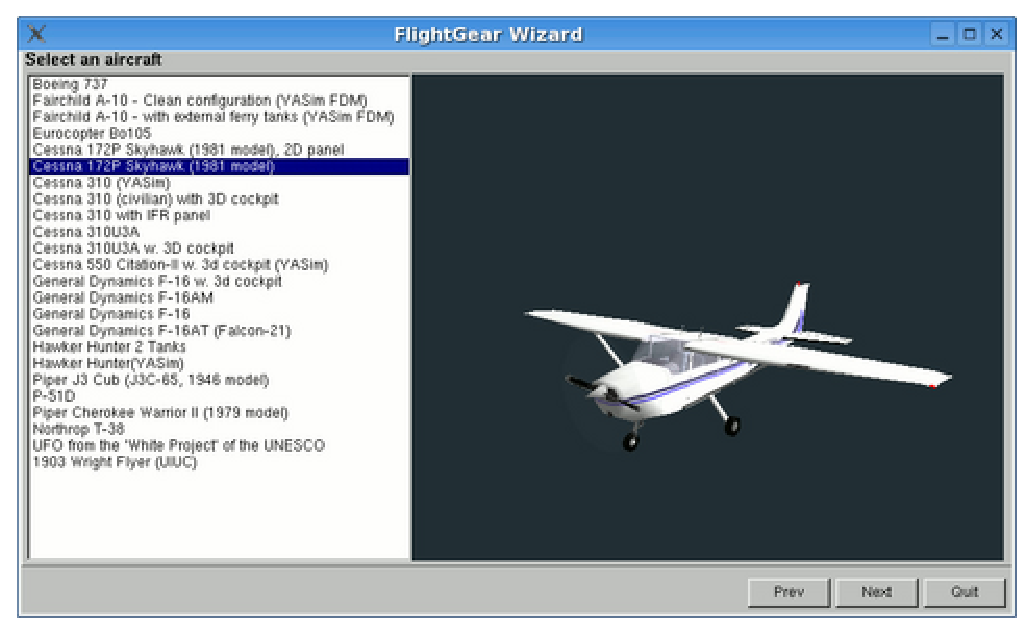
\includegraphics[width=0.5\textwidth]{img/tut_2}
\end{center}

\ifchinese
你可以从任何机场启动教程,然而我假设你使用了 FlightGear 的默认的旧金山国际机场(KSFO):
\fi
\iffalse
\IfLanguageName{english}{
You can start from any airport for this tutorial, but I will assume that you
will start from FlightGear's default airport of San Francisco (KSFO):
}{}
\fi
\IfLanguageName{french}{
Vous pouvez d\'{e}marrer de n'importe quel a\'{e}roport pour ce tutoriel, mais je partirai
du principe que vous d\'{e}marrerez de l'a\'{e}roport de San Francisco (KSFO), l'a\'{e}roport
par d\'{e}faut de FlightGear :
}{}

\begin{center}
\includegraphics[width=0.5\textwidth]{img/tut_3}
\end{center}

\ifchinese
选择好了 KSFO 之后就点\button{下一步}按钮,对模拟器来说你可以从任何时间点起飞。不过对于你的第一次飞行,我建议还是从午间起飞。另外建议你使用小一点的分辨率 $800\times600$。之后你可以再使用更高的分辨率,然而这对性能会有较大影响。按\button{运行}按钮,则会应用你的选项来启动 \FlightGear{}。
\fi
\iffalse
\IfLanguageName{english}{
Once you have selected KSFO and clicked on the \button{Next} button, you can set
any number of options for the simulator. For your first flight, I suggest
starting at noon. I would also recommend that you start with a small resolution
of $800\times600$. Later on, you can play around with the options and use a
higher resolution, but this obviously adversly affects performance. Click on the
\button{Run} button and \FlightGear{} will start with the options you
selected.
}{}
\fi
\IfLanguageName{french}{
une fois que vous avez choisi KSFO et cliqu\'{e} sur le bouton \button{Suivant}, vous pourrez
param\'{e}trer toutes les options que vous souhaitez pour le simulateur.
Pour votre premier vol, je vous sugg\`{e}re de d\'{e}marrer \`{a} l'heure
de midi. Je recommanderais \'{e}galement de d\'{e}buter avec une petite
r\'{e}solution de $800\times600$. Par la suite, vous pourrez vous amuser avec les
options et utiliser une meilleure r\'{e}solution, cependant ceci affecte la performance de
mani\`{e}re n\'{e}gative. Cliquez sur le bouton \button{D\'{e}marrer} et \FlightGear{} d\'{e}marrera avec les options que vous avez
choisi.
}{}

\begin{center}
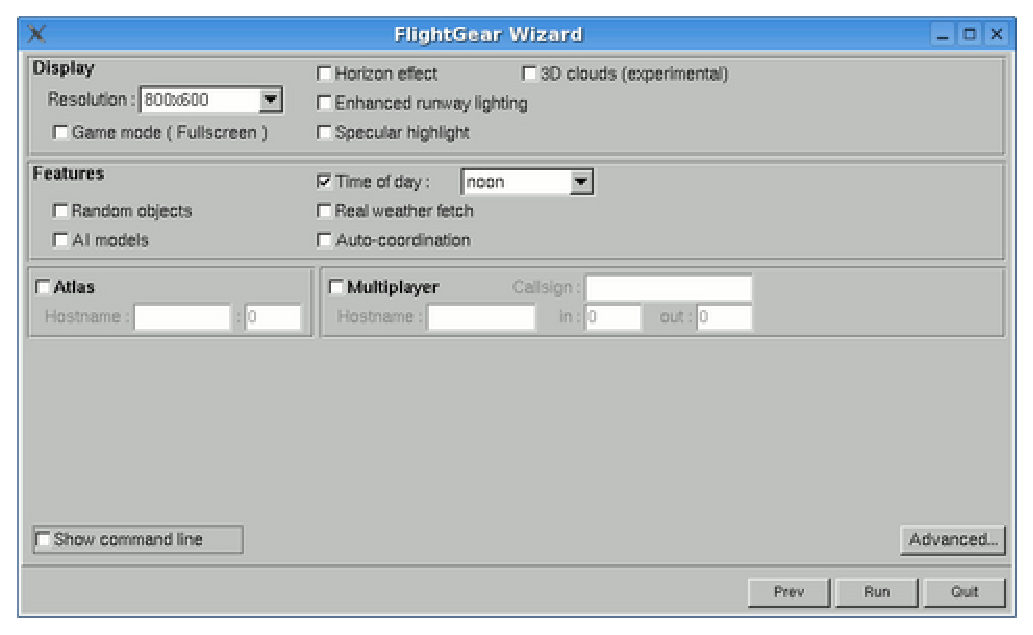
\includegraphics[width=0.5\textwidth]{img/tut_4}
\end{center}

\ifchinese
如果在你的 Windows 系统上运行最新版的 \FlightGear{} 有问题的话,可以尝试使用旧版本(比如 0.9.8)这样可以减低对显卡的需求。你可从 \FlightGear{} 下载页面找到 FTP 镜像来下载 \weblong{http://www.flightgear.org/download/}。
\fi
\iffalse
\IfLanguageName{english}{
If you have problems running the latest version \FlightGear{} on
your Windows system, you may want to try an earlier version with lower
graphics requirements (for example 0.9.8). You can find previous releases on
the FTP mirrors mentioned at the top of the \FlightGear{} download page:
\weblong{http://www.flightgear.org/download/}.
}{}
\fi
\IfLanguageName{french}{
Si vous rencontrez des difficult\'{e}s \`{a} faire fonctionner la derni\`{e}re version de
\FlightGear{} sur votre syst\`{e}me Windows, vous pourriez tender d'essayer une version
avec des pr\'{e}-requis moindres en mati\`{e}re de graphisme (comme par exemple la
0.9.8). Vous pouvez trouver les version pr\'{e}c\'{e}dentes sur les miroirs FTP
mentionn\'{e}s en haut de la page de t\'{e}l\'{e}chargement de \FlightGear{} :
\weblong{http://www.flightgear.org/download/}.
}{}

\ifchinese
如果你在 Windows Me 系统时飞行模拟器突然变得卡卡的,帧速率快速降低。可以尝试关掉所有除 Explorer 和 Systray 外的所有进程,之后再运行 \FlightGear{}。如果你关掉的进程有杀毒软件,这会带来一定的安全风险。在一台 Windows Me 的机器上,\FlightGear{} 使用 $800\times600$ 分辨率可以有较好效果,稍低一些的 $640\times480$ 会触发更低的帧速率。
\fi
\iffalse
\IfLanguageName{english}{
If you are running under Windows Me and the flight simulator suddenly starts
\index{troubles!stuttered simulation}stuttering, with the frame rate dropping,
try killing all tasks except Explorer and Systray before you
launch \FlightGear{}. If one of the tasks you kill is an antivirus or
such protection software, this is an obvious security risk. Also, on one
Windows Me machine, a \FlightGear{} of $800\times600$ yielded good results,
while a lower resolution of $640\times480$ triggered much lower FPS levels
(Frames Per Second).)
}{}
\fi

\IfLanguageName{french}{
Si vous fonctionnez sous Windows Me et que le simulateur commence soudainement
\`{a} \index{probl\`{e}mes!simulation saccad\'{e}e}saccader, avec un taux d'image
par seconde qui diminue, essayez de stopper toutes les t\^{a}ches de fond de
votre syst\`{e}me mis \`{a} part Explorer et Systray avant de lancer \FlightGear{}.
Si l'une des t\^{a}ches que vous supprimez est un antivirus ou un autre logiciel de
protection, c'est un risque de s\'{e}curit\'{e} \'{e}vident. Aussi, sur une machine
Windows Me machine, un \FlightGear{} de $800\times600$ a donn\'{e} de bons
r\'{e}sultats, alors qu'une r\'{e}solution inf\'{e}rieure de $640\times480$ donne
des niveaux de taux de d'image par seconde (FPS, Frames Per Second) bien inf\'{e}rieurs.
}{}

\ifchinese
\subsection{Linux 和其他 UNIX 系统}
\fi
\iffalse
\IfLanguageName{english}{
\subsection{Linux and other unices}
}{}
\fi

\IfLanguageName{french}{
\subsection{Linux et autres unices}
}{}

\ifchinese
在 Linux 和其他类 UNIX 系统上,也许你必须从命令行启动 \FlightGear{}。如果你已经安装了 \FlightGear{} 但在菜单里找不到的话,可以尝试:
\fi
\iffalse
\IfLanguageName{english}{
On Linux and other Unix-like systems, you may have to run \FlightGear{} from
the command line. If you have installed \FlightGear{} but cannot find it
in your menu system, try the
following:
}{}
\fi
\IfLanguageName{french}{
Sur Linux et autres syst\`{e}mes bas\'{e}s sur Unix, vous pourriez avoir \`{a} d\'{e}marrer \FlightGear{} \`{a} partir de
la ligne de commande. Si vous avez install\'{e} \FlightGear{} mais que vous ne parvenez pas \`{a} le trouver dans le menu
de votre syst\`{e}me, essayez la proc\'{e}dure suivante :
}{}

\ifchinese
\begin{itemize}
\item 在命令行窗口下输入命令 \command{fgrun}。如果安装的话,会启动一个和 Windows 下一样的图形化向导。

\item 除此之外,还可以打开命令行窗口输入如下命令:
\command{fgfs -$ $-timeofday=noon -$ $-geometry=800x600}.
\end{itemize}

\fi
\iffalse
\IfLanguageName{english}{
\begin{itemize}
  \item From a terminal window (also named ``console'' window) try
  running the  \command{fgrun} command. If installed, this will run the same
  GUI Wizard as under Windows as described above.

    \item Alternatively, open a terminal window and type the following command:
  \command{fgfs -$ $-timeofday=noon -$ $-geometry=800x600}.
\end{itemize}
}{}
\fi
\IfLanguageName{french}{
\begin{itemize}
  \item A partir d'une fen\^{e}tre de terminal (appel\'{e}e aussi fen\^{e}tre ``console'', essayez
  de lancer la commande \command{fgrun}. Si elle est install\'{e}e, vous obtiendrez le m\^{e}me assistant
  que sous Windows comme d\'{e}crit ci-dessus.

    \item Sinon, ouvrez une fen\^{e}tre de terminal et entrez la commande suivante :
  \command{fgfs -$ $-timeofday=noon -$ $-geometry=800x600}.
\end{itemize}

}{}

\ifchinese
\subsection{黑夜里?}

如果没有命令行选项 \command{-$ $-timeofday=noon},\FlightGear{} 会按旧金山当前时间(对欧洲来说通常是晚间)来启动。要改变模拟器的时刻,只需要在 \button{Environment->Time Settings} 菜单里选择 \button{Noon} 即可。
\fi
\iffalse
\IfLanguageName{english}{
\subsection{In the dark?}

Without the \command{-$ $-timeofday=noon} option, \FlightGear{} will start at the
current time in San Francisco - often night-time if you are in Europe. To
change the time of day in the simulator to daytime, select
\button{Environment->Time Settings} from the menu and select \button{Noon}.
}{}
\fi
\IfLanguageName{french}{
\subsection{Dans le noir ?}

Sans l'option de commande \command{-$ $-timeofday=noon}, \FlightGear{} se lancera \`{a} l'heure actuelle
de San Francisco - qui correspond souvent \`{a} la nuit si vous \^{e}tes en Europe. Pour changer l'heure
du jour dans le simulateur et retrouver la lumi\`{e}re, choisissez
\button{Environnement->Param\`{e}tres horaires} \`{a} partir du menu et choisissez \button{Noon}.
}{}

\begin{center}
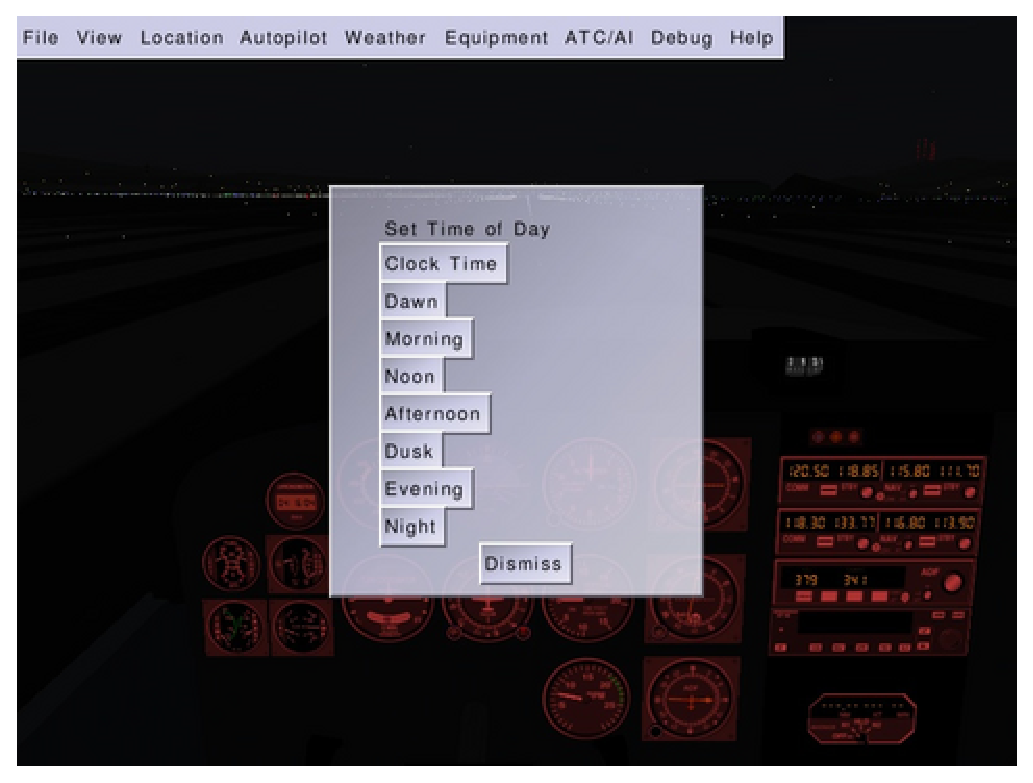
\includegraphics[width=0.5\textwidth]{img/tut_5}
\end{center}
\ifchinese
如果从菜单启动 \FlightGear{}(比如 KDE 或 GNOME),你能编辑 FlightGear 的启动图标属性,并修改 \command{fgfs} 命令到类似 \command{fgfs -$ $-timeofday=noon -$ $-geometry=1024x768},或者加入任何你想加入的命令行选项。有关命令行选项相关内容可以参考第 ~\ref{takeoff} 章\textit{起飞:如何启动程序}。
\fi
\iffalse
\IfLanguageName{english}{
If running \FlightGear{} from a menu (e.g. under KDE or Gnome), you can edit the
FlightGear launch icon properties and change the simple \command{fgfs} fgfs
command to something like \command{fgfs -$ $-timeofday=noon -$ $-geometry=1024x768},
or include whatever command options you wish. Further details of the command
line options can be found in Chapter~\ref{takeoff},
\textit{Takeoff: How to start the program}.
}{}
\fi
\IfLanguageName{french}{
Si vous utilisez \FlightGear{} \`{a} partir d'un menu (par ex. sous KDE ou Gnome), vous pouvez \'{e}diter les
propri\'{e}t\'{e}s de l'ic\^{o}ne de lancement de FlightGear et modifier la commande simple \command{fgfs}
vers quelque chose comme \command{fgfs -$ $-timeofday=noon -$ $-geometry=1024x768},
ou inclure toute option de commande que vous souhaitez. Plus de d\'{e}tails sur les options de ligne de
commande peuvent \^{e}tre trouv\'{e}s dans le chapitre ~\ref{d\'{e}collage},
\textit{D\'{e}collage : comment d\'{e}marrer le programme}.
}{}

%%%%%%%%%%%%%%%%%%%%%%%%%%%%%%%% CHINESE VERSION %%%%%%%%%%%%%%%%%%%%%%%%%%%%%%%%%%%%%%%%%%%%%%

\ifchinese
\section{第一个挑战——直线平飞}\label{sec:FlyingStraight}

当 \FlightGear{} 启动以后,你会看到如下的窗口并听到发动机的声音:

\begin{center}
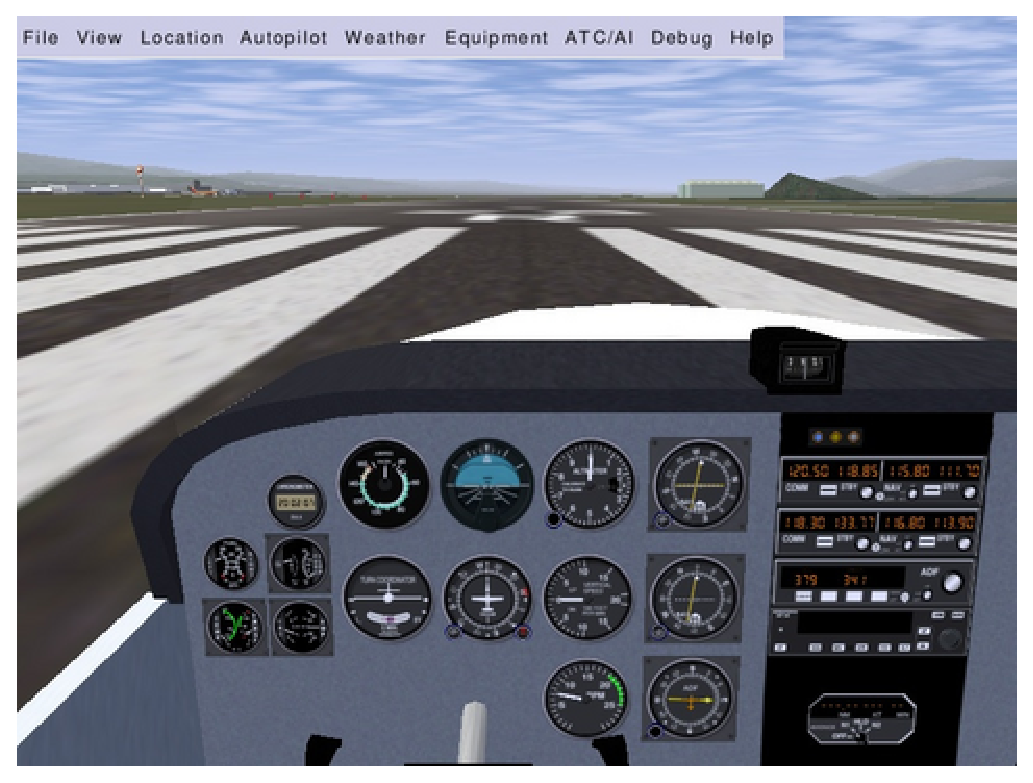
\includegraphics[width=0.5\textwidth]{img/tut_6}
\end{center}

启动时,飞机停在跑道的起点且发动机维持低功率运转。飞机也许会轻微抖动,但不会移动。

\subsection*{关于键盘控制}\index{键盘}

\begin{itemize}
    \item 在本教程中,小写字母表示你只需要按这个键即可,大写意味着你需要同时按 \textcolor{blue}{\key{$\Uparrow$~Shift}} 键和这个键。也就是说,如果你看到“v”键表示你只需要按字母 \key{v} 即可,如果你看到“V”则意味着你需要按下 \key{Shift} 键的同时按字母 \key{v}。\index{键盘!大写和小写键}(简单来说, V 就代表\key{Shift-v})
    \item 本教程假设你已经的 \key{NumLock} 是打开状态。键盘右上角的绿灯亮起。如果没亮,按\textcolor{green}{\key{NumLock}}键直到绿灯亮起。
    \end{itemize}

\begin{center}
\includegraphics[width=0.5\textwidth]{img/tut_7}
\end{center}
    
\index{视图!改变}

按 \key{v} 键来从外面查看飞行器。重复按 v 键可以循环各种视图模式,直到你回到驾驶舱中。按 \key{V} 将会反向循环。

\begin{center}
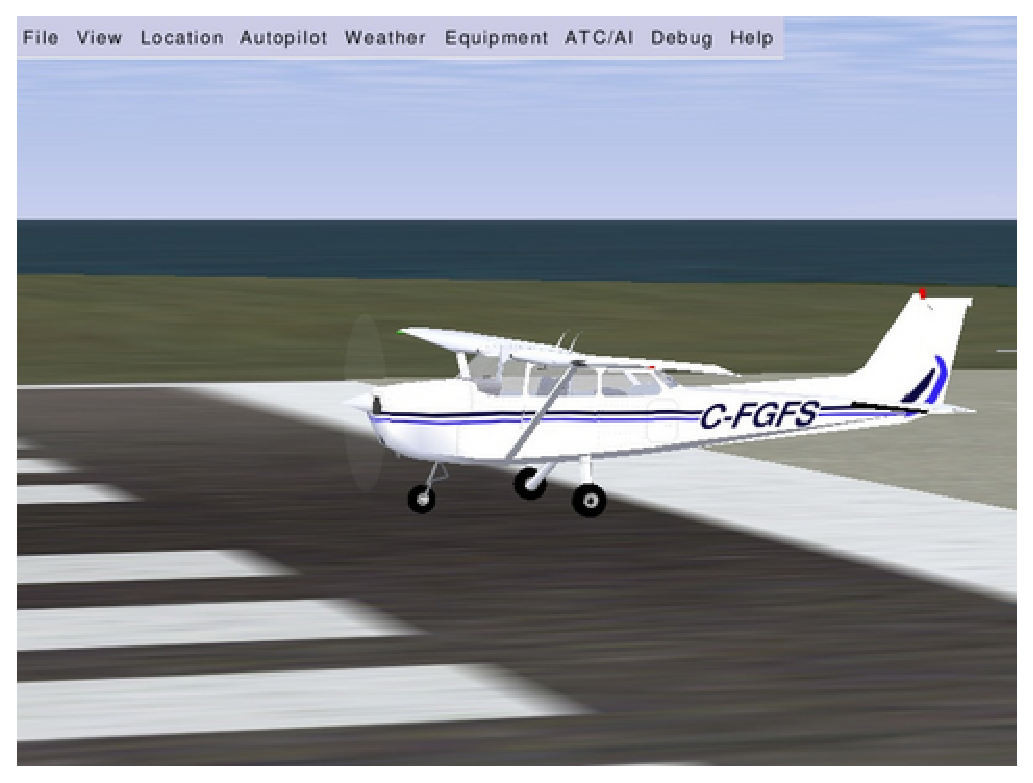
\includegraphics[width=0.5\textwidth]{img/tut_8}
\end{center}

在真实中,我们会围着飞机转一圈检查所有都正常,没有任何东西阻碍移动控制面,也没任何堵住仪器的开口处。而在模拟器里,这些都已经在启动前帮我们做好了。

按住 \key{Page Up} 大概八秒,你能听到发动机的声音越来越大。

飞机开始在跑道上加速。在离地之前,飞机会被拉向左侧,并向左侧倾斜,并坠毁在地面上(也许)。

\index{视图!即时回放}

你可以通过 \button{View -> Instant Replay} 来检查整个坠毁过程的回放。按对话框底部的 \button{Replay} 按钮,下面这张图就是坠毁时的状态。你按 \key{F3} 可以截图保存。你可以用 \key{F10} 来切换菜单是不是显示。

\begin{center}
\includegraphics[width=0.5\textwidth]{img/tut_9}
\end{center}

之后,你可以用 \button{File->Quit} 退出 \FlightGear{} 并用与之前同样的选项重新进入模拟器。

为了能够直线飞行,你需要控制飞机的\Index{驾驶盘}:

\begin{center}
\includegraphics[width=0.5\textwidth]{img/tut_10}
\end{center}

你可以用游戏杆控或者鼠标来控制。要使用鼠标你需要将鼠标置于控制模式,可以通过按 \key{Tab} 键直到指针变成 $+$ 形。移动鼠标就可以看到驾驶盘也在随之移动。按 \key{v} 键可以从外面观察飞机。此时继续移动鼠标,可以看到机尾的升降舵和机翼后部的副翼也在移动。如果你的视点离飞机太远,看不清楚的话,可以按几次 \key{x} 键来放大,按 \key{X} 来缩小。\key{Ctrl-x} 可以恢复默认的缩放级别。此时按 \key{V} 回到驾驶舱里。

按 \key{Tab} 几次直到鼠标进入观察模式。在此模式下,鼠标指针会变成 $\leftrightarrow$ 形。这可以允许你更容易的移动鼠标环顾四周。按鼠标左键将会重新回到中间。你可以在控制模式时临时进入观察模式,只需要按住鼠标右键并移动鼠标。最终再按 \key{Tab} 会回到正常鼠标模式。

简单来说,\key{Tab} 让鼠标在三个模式之间循环:
\begin{itemize}
    \item \textit{正常模式}\index{鼠标!正常模式}。此模式让你可以点击菜单或点击仪表板。
    \item \textit{控制模式}\index{鼠标!控制模式}\index{驾驶盘!鼠标控制模式}。 此时鼠标控制驾驶盘(指针是 $+$ 形)。
    \item \textit{查看模式}\index{鼠标!查看模式}。此时鼠标控制观察的角度(指针是 $\leftrightarrow$ 形)。
\end{itemize}

现在尝试在起飞,按 \key{Tab} 进入控制模式。按住 \key{Page Up} 键将发动机油门推到最大功率,不要强制通过鼠标让其在跑道上保持直线,就让它这样向左滑行直到自己升入空中。然后用鼠标尝试让飞机保持直线平飞。(如果你想控制在地面的飞机,请查看 \ref{sec:TaxiTurning} 小节)。

你会发现你需要防止飞机向左滚转:

\begin{center}
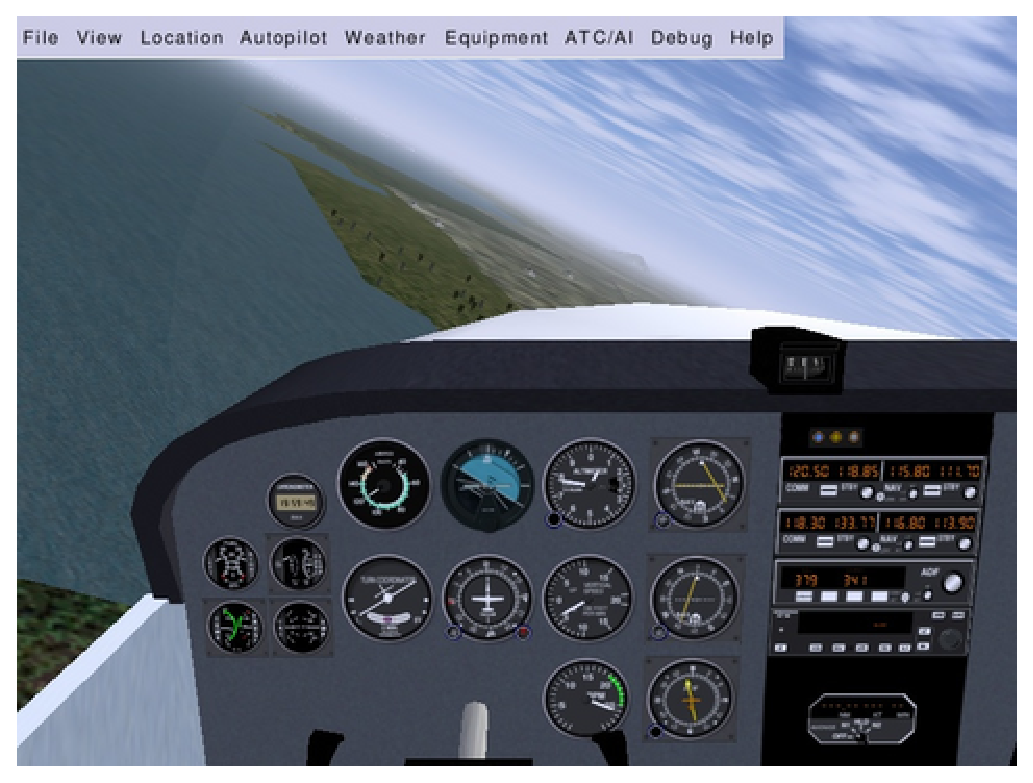
\includegraphics[width=0.5\textwidth]{img/tut_11}
\end{center}

……或者向右滚转:


\begin{center}
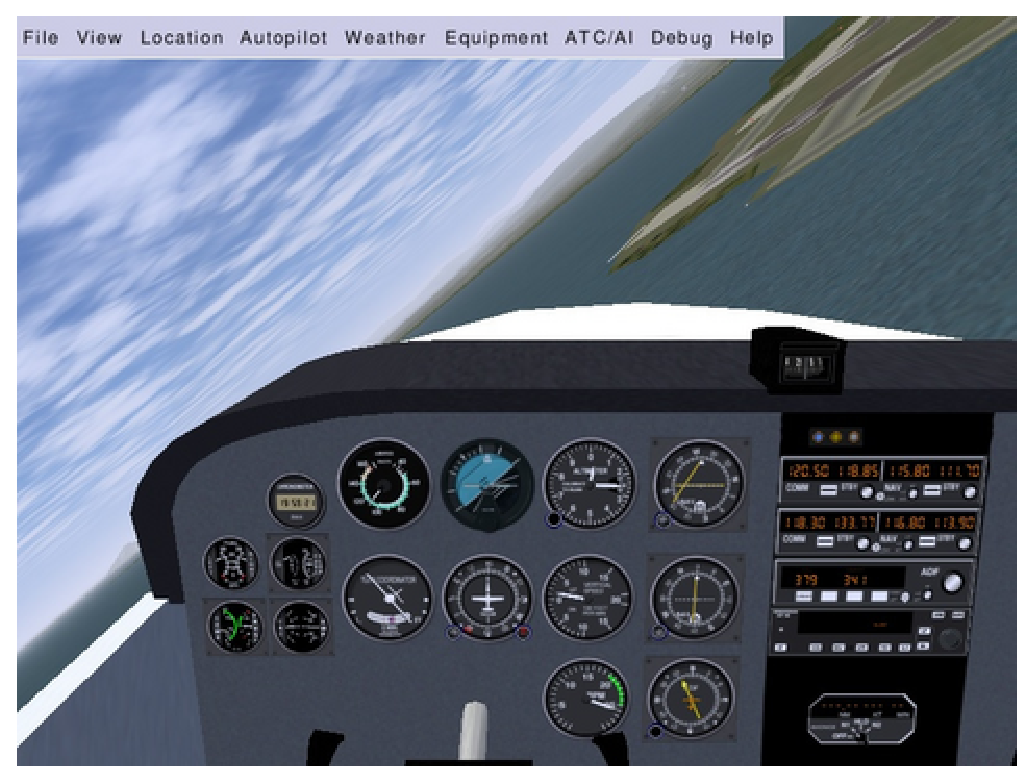
\includegraphics[width=0.5\textwidth]{img/tut_12}
\end{center}

……或者向地面扎去:


\begin{center}
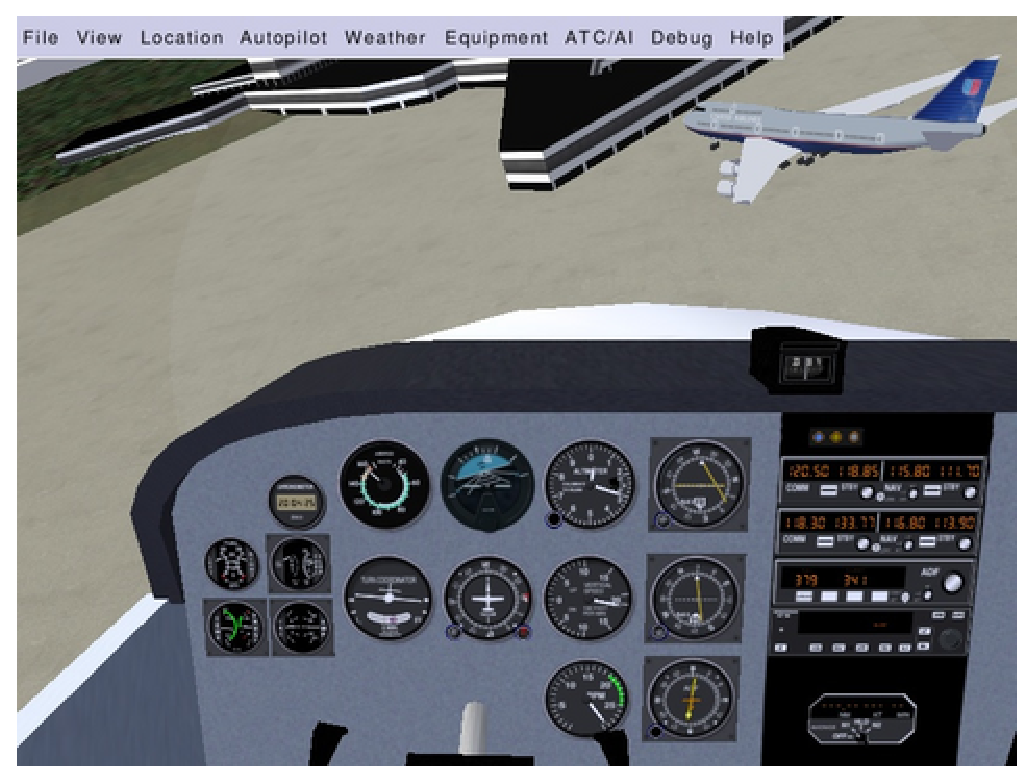
\includegraphics[width=0.5\textwidth]{img/tut_13}
\end{center}

尽可能的沿直线飞行,让地平线稍稍高于机头:

\begin{center}
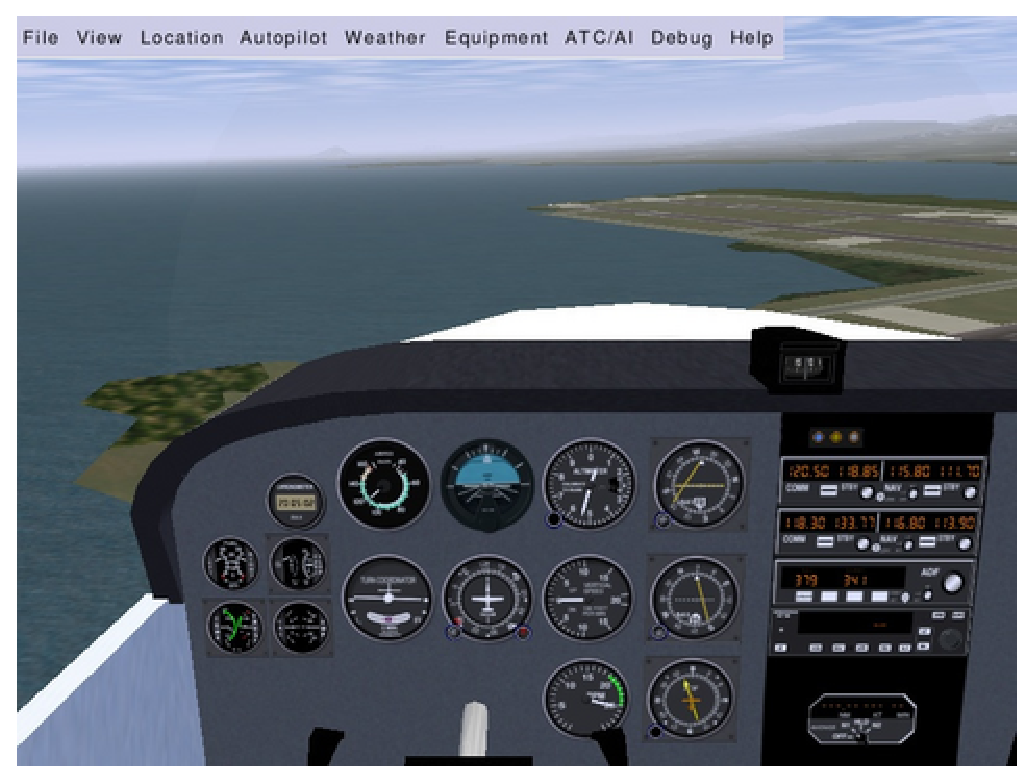
\includegraphics[width=0.5\textwidth]{img/tut_15}
\end{center}

无论你在电脑游戏或模拟游戏方面的能力如何,第一次飞行很可能不会成功。飞机可能会坠毁,也许只在起飞后不久。这也就是为什么很多人对真实性比较高的飞行模拟感到绝望。只需要多多尝试,也许你会找到一种很舒适的控制方式。

\index{驾驶盘!拉杆}
一个普遍的错误是向前移动鼠标,以使机头向上昂起。实际上,你需要向后移动鼠标这样才能让驾驶盘向后拉杆。

同样的,当你想要降低飞机的机头,你需要向前移动鼠标。也许这有些奇怪,不过所有飞机都是按照这种方式来控制的。随着时间的推移,你会明白这种方式的好处。\index{问题!鼠标速度}你也许会发现鼠标的小幅移动会对飞机有很大的影响,所以也许降低鼠标的敏感度会有一些帮助。

如果你需要可视化一些的话,这么说也许会一些帮助:假设在你桌子上有一个美式橄榄球,而你的手必须“粘在”球的顶端。如果你要向前移动,则球就会向前滚动,而你的手指则会碰到桌面。如果你向后移动手指,则球会向后滚动,而你的手指就会指向天花板。你的手就是飞机:

\begin{center}
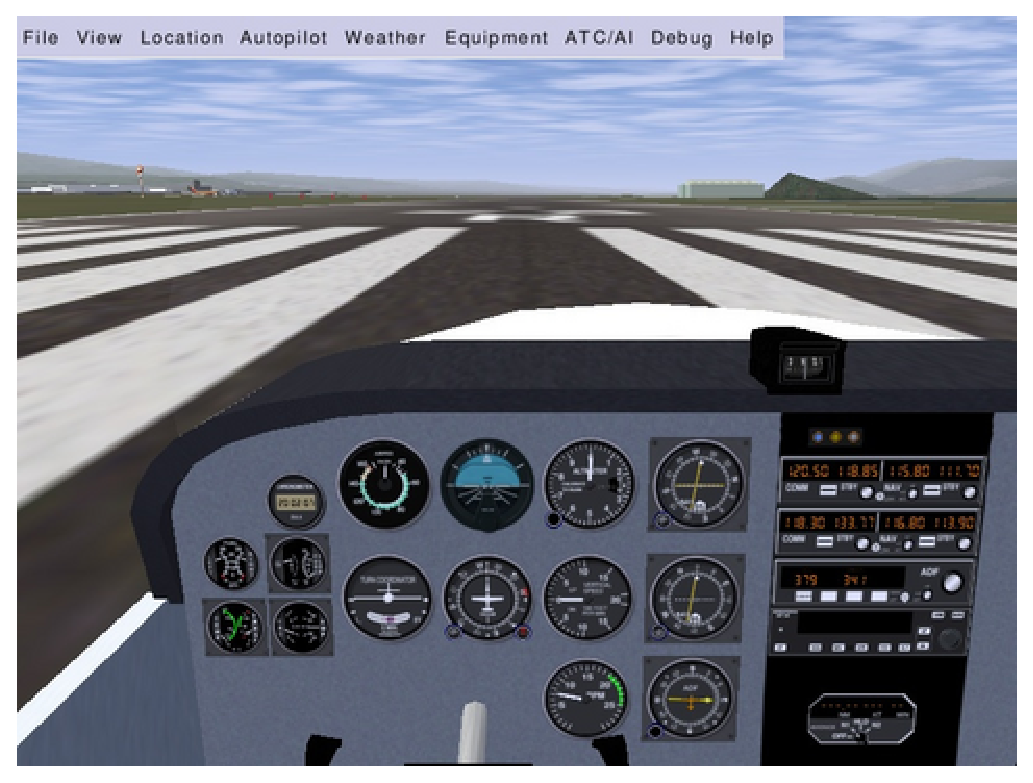
\includegraphics[width=0.5\textwidth]{img/tut_6}
\end{center}

另一个普遍的错误是假设驾驶盘的动作与飞机的滚转坡度一致。也就是说,你认为只要驾驶盘水平,飞机也会平飞。这并非如此,驾驶盘知识控制飞机滚转的\emph{速率}。如果飞机有向左 20$\textdegree$ 的坡度,而驾驶盘是水平的,则意味着飞机会保持向左 20$\textdegree$ 的坡度直到外力改变这个状况。如果想要让飞机恢复平飞,需要温柔的向右转动驾驶盘(温柔的向右移动鼠标),并稍稍维持向右一段时间。飞机会向右慢慢滚转。当与地平线平齐时,再将驾驶盘慢慢转平。飞机会保持平飞(直到外力来改变其方位)。

第三个错误是尝试找到驾驶盘/鼠标的“正确位置”。很自然的,你想找到一个完美的位置,可以让飞机保持直线平飞。事实上没有这种里想的驾驶盘位置。飞机本质上在空中是不稳定的,你需要不断的用鼠标做小幅移动,来修正飞机的姿态并保持直飞。也许刚开始会让你耗费全部注意力。这就如同开车,让飞机保持直线平飞将很快会变成一种本能。对长期的飞行来说,你还可以偶尔使用自动驾驶仪来保持平飞,然而本教程将不会涉及。

为了帮助你找到控制的感觉,眼睛始终关注着窗外景物,而不要叮着驾驶盘或仪表板。检查地平线与机头之间的高度差,地平线和你飞机的发动机盖子是你的主要仪表。只有每隔一段时间扫一眼仪表板而已。

在鼠标处于控制模式时\index{驾驶盘!鼠标控制模式}时,千万不要将鼠标移出 FlightGear 窗口边缘以外。一旦鼠标离开窗口,就会停止控制飞机,很可能会造成极糟糕的动作!如果你想在窗口外使用鼠标,首先按 \key{Tab} 键两次切换到正常模式。

你可以使用键盘上的 \key{方向键} 来控制驾驶盘,或者使用小键盘上的 \key{8}、\key{2}、\key{4} 和 \key{6} 键。也许最开始这种方式会比鼠标控制来的简单一些,飞行时的微调控制却不如鼠标,因此持续练习鼠标控制才是王道。

也许你在机场附近飞行时,会听到蜂鸣器的声音,这是降落辅助信号\index{降落!辅助信号}。现在不用担心这些声音。

你会想了解在掌握了这些以会如何爬升。下一步要学习如何维持高度,或者在你的控制下缓慢上升和下降。

让飞机保持一个高度需要观察高度表,并通过前后小幅移动鼠标来让飞机停止上升或下降。

\index{高度表 Altimeter}高度表位于仪表板的中上部,长表针表示百英尺,短表针表示千英尺。下面这张图里的高度表示意的是 300 英尺,约 100 米\footnote{1 英尺 = 12 英寸 = 0.3048 米。口算时可以简单将英尺数除以 3,即得公制米数。——译者注}。

\begin{center}
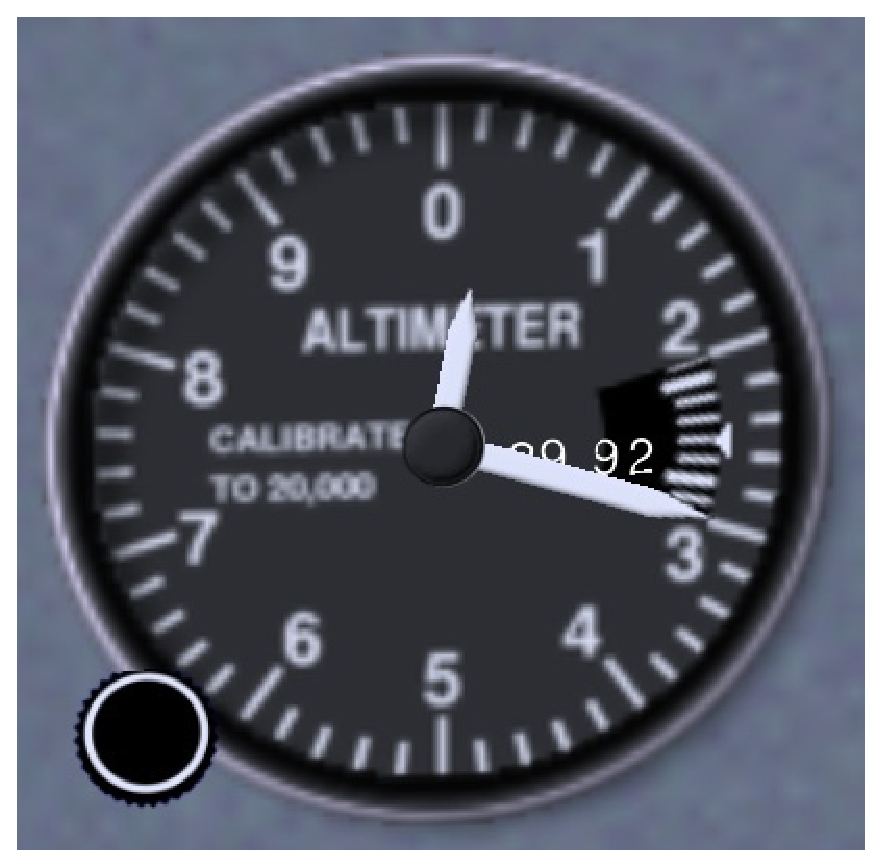
\includegraphics[width=0.25\textwidth]{img/tut_17}
\end{center}

上升或下降时高度表会作出反映,表针逆时针转表示下降,顺时针表示高度增加。如果你看到高度表“狂转”,说明你在丢高度,缓慢向后移动鼠标拉起机头即可。

一段时间以后你会发现,当平飞的时候,机头与地平线的相对位置永远是一样的。这就是平飞时的飞机姿态。让机头处在这个位置,你就几乎可以让飞机进入平飞而不需要参考任何仪表。现在你可以微调高度了。

谨记:高度表不会自动显示距海平面的绝对高度\index{高度!绝对高度}。你需要调整其与当地的气压相匹配。高度表左下角的黑色旋钮让你可以调整高度表拨正值\index{高度表!拨正值}。启动 \FlightGear{} 以后一直待在地面上,点击(鼠标在正常模式)这个黑色的旋钮,点击左侧可以让旋钮数值变小,点击右侧则会变大。使用这个小旋钮调整到当前高度。前提是你确信当前的高度。例如你在 1100 英尺,那么就调整旋钮,让高度表显示 1100 英尺。使用鼠标中键点击可以让旋钮旋转更快,或者你可以用鼠标滚轮。\key{Ctrl}-\key{c} 可以将可点击的区域高亮化。

为了让设置高度表更简单,机场会将其高度通过各种方式告知出来。也许会通过无线电服务(美国称之为 ATIS\footnote{ATIS 是 Automatic Terminal Information Service 的缩写,意为”自动终端情报服务“,中国大陆称为“情报通播”。机场在一个单独的无线电频率上广播,包括主要的与飞行相关的信息,如天气、可用跑道、气压及高度表拨正值等信息。——译者注,摘自中文维基百科})广播当前的修正海平面气压。单位是英尺汞柱(inHg)。高度表上有一个比例尺,高度表会利用拨正值来计算高度,你可以通过旋钮设置高度表拨正值\footnote{除美洲外,修正海平面气压的单位在欧洲和亚洲一般使用的是百帕(hPa)为单位。标准大气压是 1013.25 百帕,也就是 29.92 英尺汞柱。1 inHg = 33.86 hPa。设置高度表拨正值时,一般忽略小数点。这是高度表拨正值换算速查表:\web{http://www.pcwp.com/mb_conversion.html}。——译者注}。另外,如果你在地面上并知道当前机场的高度值,你也可以直接调节高度表直到其显示正确的高度。

\begin{center}
\includegraphics[width=0.25\textwidth]{img/tut_18}
\end{center}

注意,“距地面高度”和“距海平面高度”有非常大的不同。如果你在珠穆朗玛峰以距离平均海平面高度(Above Mean Sea Level,AMSL) 24000 英尺飞行,你距地面的高度(Above Ground Level,AGL)则会小很多。因此了解自己距离周边地面的高度,显然很有帮助。

\section{基本转弯}
\label{sec:InFlightTurning}



\fi

%%%%%%%%%%%%%%%%%%%%%%%%%%%%%%%% ENGLISH VERSION %%%%%%%%%%%%%%%%%%%%%%%%%%%%%%%%%%%%%%%%%%%%%%%
%\iffalse
\section{The First Challenge - Flying Straight}
\label{sec:FlyingStraight}

Once \FlightGear{} is started you will see the following window and hear the
sound of an engine:

\begin{center}
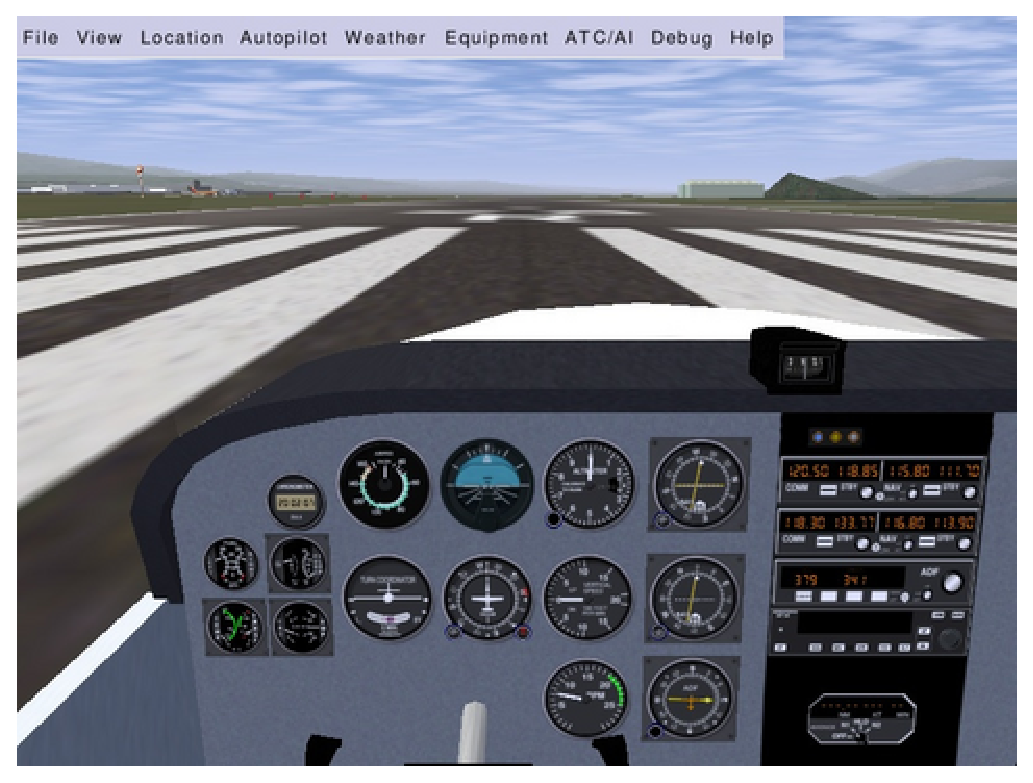
\includegraphics[width=0.5\textwidth]{img/tut_6}
\end{center}

On startup, the aircraft is at the end of the runway with the engine running
at low power. The airplane will occasionally tremble a little, but it won't
move.

\subsection*{About the keyboard.}\index{keyboard}

\begin{itemize}
    \item In this tutorial, a lowercase key letter indicates you should simply
  press that key. An uppercase means you must press shift and that key.
  (The \textcolor{blue}{\key{$\Uparrow$~Shift}} keys are those two keys with
  a hollow fat arrow pointing upwards.) In other words: if you are told to type
  ``v'', simply hit the \key{v} key briefly.
  \index{keyboard!uppercase and lowercase keys} If you are told to type ``V'',
  press the \key{Shift} key down and while you have it pushed down, hit the
  \key{v} key, then release the \key{Shift}  key. (In short: V is the same as
  \key{Shift-v}.)
    \item The tutorial will assume you have the \key{NumLock} switched on.
  \index{keyboard!numeric} When switched on, you should find a small green
  light on at the right of your keyboard. Press the
  \textcolor{green}{\key{NumLock}} key repeatedly until the lamp is on.
\end{itemize}

\begin{center}
\includegraphics[width=0.5\textwidth]{img/tut_7}
\end{center}

\index{view!changing}
Press \key{v}, to view the aircraft from the outside. Type v repeatedly to
scroll through a number of different views until you return to the cockpit.
Typing \key{V} will cycle backwards through the views.):

\begin{center}
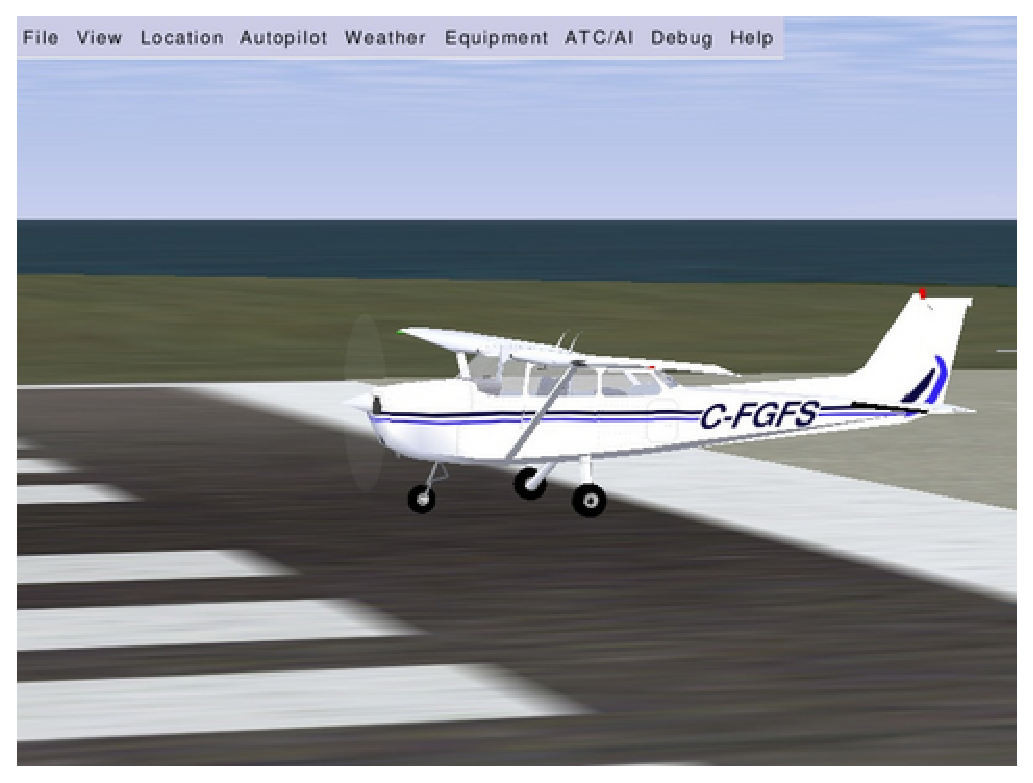
\includegraphics[width=0.5\textwidth]{img/tut_8}
\end{center}

In real life, we would have inspected the airplane all around to check
everything is working, nothing is hampering the moving parts,
and nothing is obstructing the instrument openings. In the simulator, this is
already done for us before we start.

Hold the \key{Page Up} key down for about eight seconds. You will
hear the engine sound rise.

The airplane will start accelerating down the runway. As it does so, it will
drift to the left, before finally taking off, banking to the left,
falling to the ground and crashing (probably).

\index{view!instant replay}
You can see a replay of the crash using the  \button{View -> Instant Replay}
menu. Click the \button{Replay} button at the bottom of the dialog window, then
use \key{v} and \key{V} to see the airplane from the outside. The
picture below shows the end part of the flight. You can take a snapshot by
typing the \key{F3} key.
You can also use the \key{F10} key to toggle the menu bar on or off.

\begin{center}
\includegraphics[width=0.5\textwidth]{img/tut_9}
\end{center}

Having observed your crash, exit from \FlightGear (using \button{File->Quit})
and restart the simulator using the same options as before.

In order to fly straight you need the airplane's control\index{yoke} yoke:

\begin{center}
\includegraphics[width=0.5\textwidth]{img/tut_10}
\end{center}

You can control the yoke using a joystick, or by moving the mouse. To use the
mouse you need to be in mouse yoke mode. Get in that mode by pressing \key{Tab}.
The mouse cursor becomes a $+$ sign. Move the mouse and see the
yoke moving accordingly. Type \key{v} to see the plane from the outside. If you
move the mouse again you will see the tail elevator and the ailerons at both
wings ends move. If your viewpoint is too far from the aircraft to see any
movement, type \key{x} a few times to zoom in.
Type \key{X} to zoom back out. \key{Ctrl-x} returns the view to the default zoom
level. Type \key{V} to change the view back to the cockpit.

Pressing \key{Tab} again gets you in mouse view mode. In this mode the mouse cursor will
be a $\leftrightarrow$. sign. This allows you to look around easily by moving
the mouse. Clicking the left mouse button will re-center the view.  You can also
change your view direction in the normal and yoke modes by holding down the right
mouse button and moving the mouse. A further press of \key{Tab} will return you to the
normal mouse mode.

To summarize, the \key{Tab} key cycles the mouse through three modes:
\begin{itemize}
    \item \textit{Normal mode}\index{mouse!normal mode}. This mode allows you to
  click on the menu and on the instrument panel.
    \item \textit{Yoke mode}\index{mouse!yoke mode}.\index{yoke!mouse yoke mode}
  The mouse controls the yoke (+ pointer shape).
    \item \textit{View mode}\index{mouse!view mode}. The mouse controls the
  view direction ($\leftrightarrow$ pointer shape).
\end{itemize}

Try taking off again using the mouse to control the yoke. Press \key{Tab} to put
the mouse in yoke mode ($+$pointer shape) and raise the engine throttle to
maximum by holding the \key{Page Up} key down. Do not try to keep the airplane
rolling straight on the runway using the mouse/yoke. Let it drift leftwards.
Wait till it rises in the air. Then use the mouse to try and get the
airplane to fly straight. (If you want to control the airplane on the
ground see section \ref{sec:TaxiTurning}.)

You will find that you must prevent the airplane from banking to the left:

\begin{center}
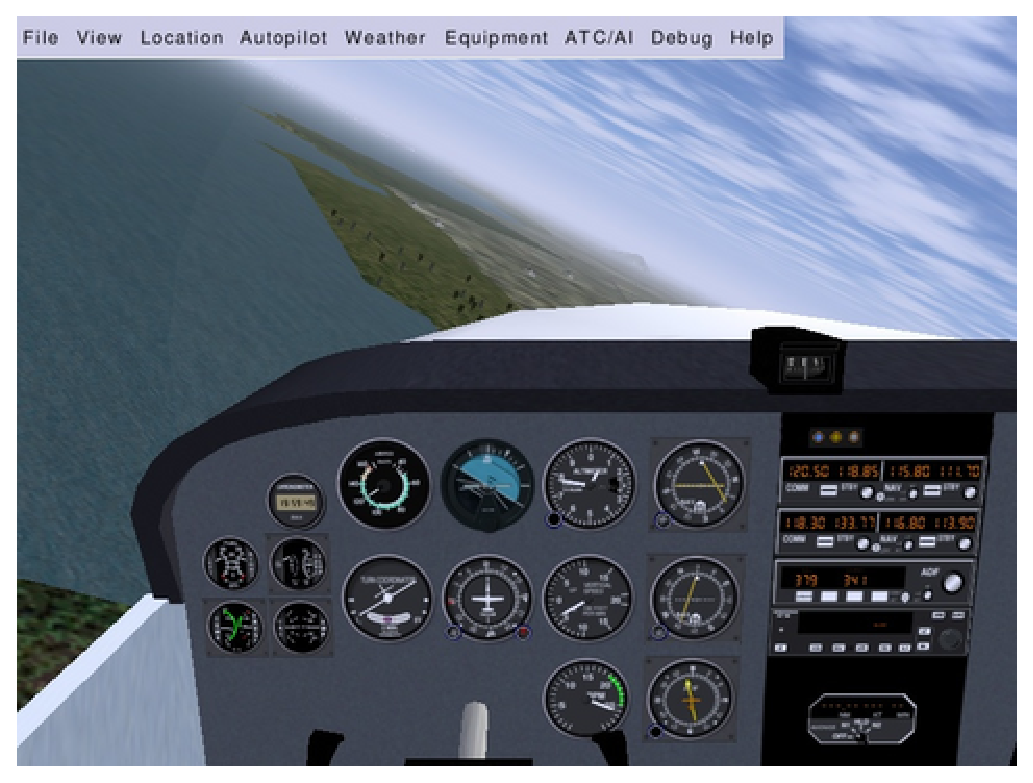
\includegraphics[width=0.5\textwidth]{img/tut_11}
\end{center}

... or to the right:


\begin{center}
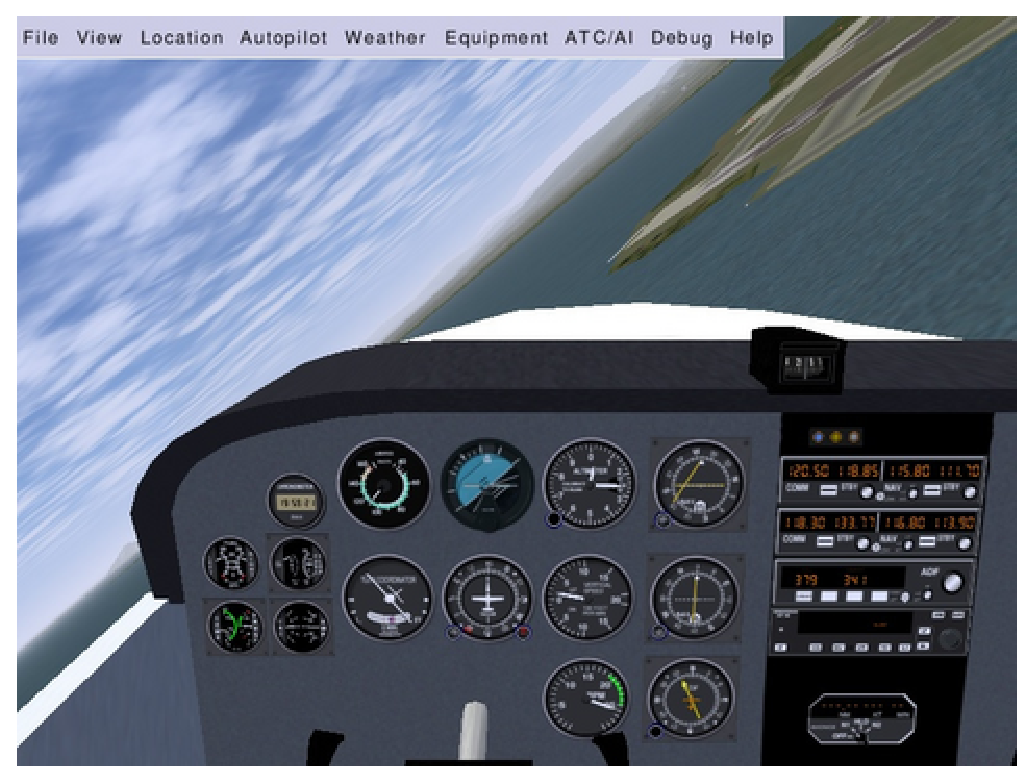
\includegraphics[width=0.5\textwidth]{img/tut_12}
\end{center}

... or from plunging to the ground:


\begin{center}
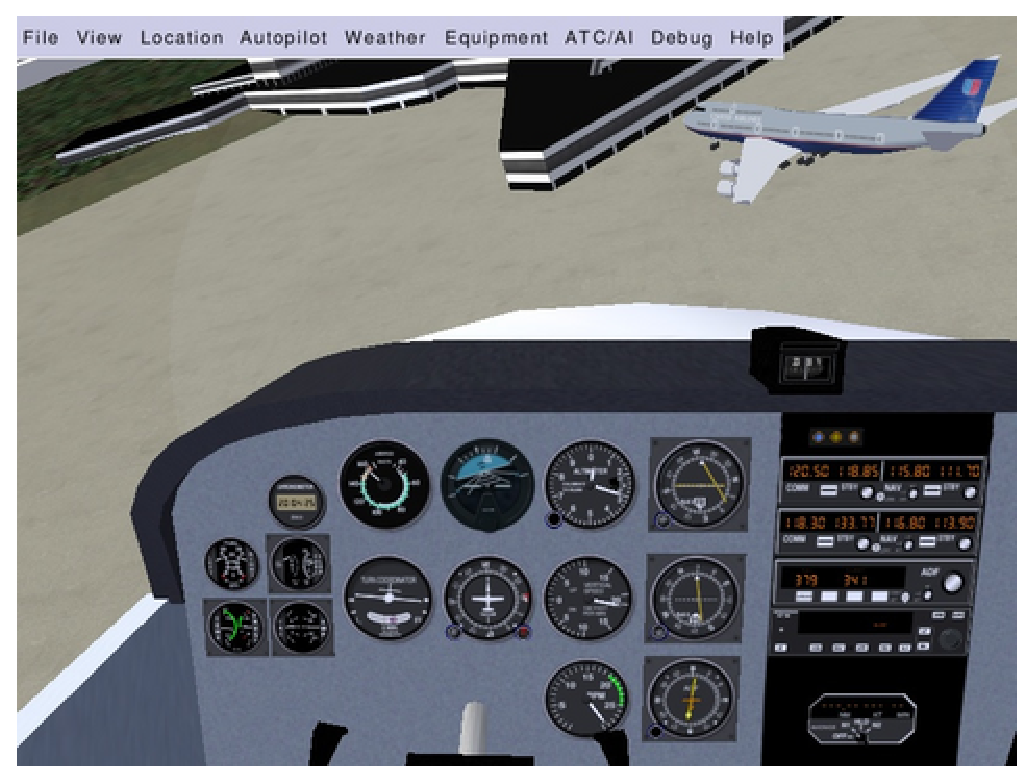
\includegraphics[width=0.5\textwidth]{img/tut_13}
\end{center}

Try to fly more or less straight, with the horizon stable slightly above the
airplane nose:

\begin{center}
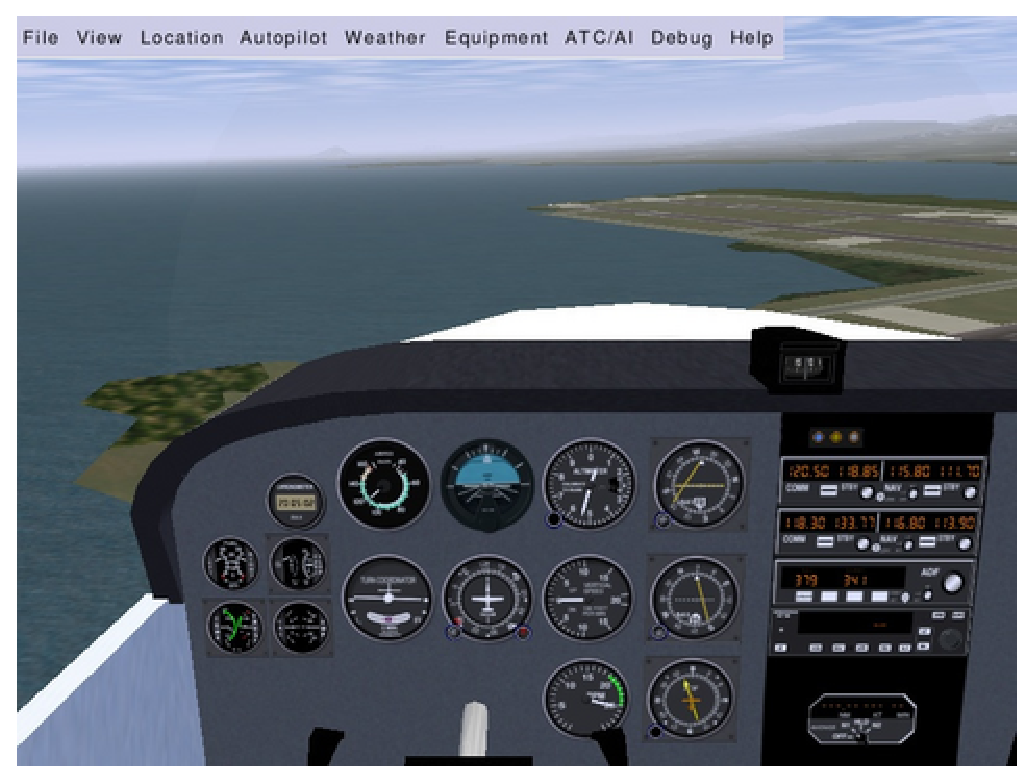
\includegraphics[width=0.5\textwidth]{img/tut_15}
\end{center}

Whatever your skills at video games or simpler simulators, you will probably
not succeed at first. The airplane will crash, probably quite soon after
take-off. This is the moment where most candidates get desperate and abandon
trying to fly a simulator or a real aircraft. Just hold tight and keep trying.
Eventually you will develop a feel for the subtle control inputs required.

\index{yoke!pulling}
The most common error is moving the mouse forwards to bring the nose up. In
fact, you must pull the yoke by moving the mouse backwards to do this.

Equally, when you want to lower the airplane's nose, you must move
the mouse forwards. This can seem odd, but all airplane control yokes
are designed that way. With time, you will wonder how you every thought it
worked any other way. \index{troubles!mouse speed} You will also find that
small mouse movements have a large effect on the aircraft. You may find that
decreasing your mouse sensitivity may help initially.

If you have difficulty visualising this, the following analogy may help.
Imagine a soccer ball is on your desk and you have ``glued'' your hand
to the top of it. If you move your hand forwards the ball will roll forwards
and your fingers will point to to the desk. If you move your hand backwards the
ball will roll  back and your fingers will now point up at the ceiling.
Your hand is the airplane:


\begin{center}
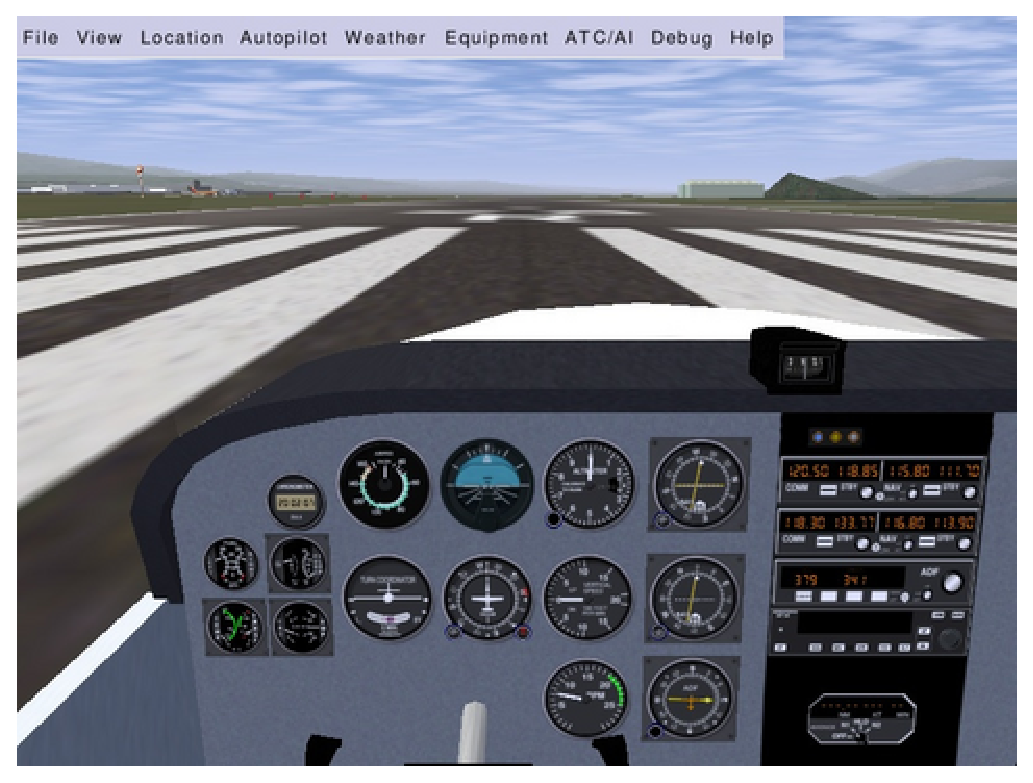
\includegraphics[width=0.5\textwidth]{img/tut_6}
\end{center}

Another common error is the assumption that the control inputs directly
match airplane bank. In other words, you believe if the control yoke is
level, the airplane will fly level. This is not true. The yoke
controls the \emph{rate} at which the airplane banks. If the airplane is
banked 20$\textdegree$ to the left and the control yoke is level, the
airplane will stay banked at 20$\textdegree$ left until some other force
affects it. If you want to return the airplane to level flight, you have to
turn the control yoke slightly to the right (move the mouse slightly
rightwards) and keep it slightly to the right for a while. The airplane
will turn slowly rightwards. Once it is level with the horizon, bring the
control yoke level too. Then the airplane will stay level (until some other
force changes its orientation).

A third error is trying to find ``the right position'' for the
yoke/mouse. Naturally, you will want to find the fine tuning that will leave
the airplane fly straight. Actually there is no such ideal yoke
position. The airplane is inherintely unstable in the air. You must constantly
correct the airplane's attitude and keep it flying straight with tiny movements
of the mouse. This may seem to take all your concentration intially,
but just like driving a car, keeping the aircraft straight and level will soon
become second nature. For longer flights, you will eventually use the autopilot
to keep the airplane level, but this is outside the scope of this tutorial.

To help fine-tune your senses to the control inputs required, keep your eyes on
the outside scenery and not get fixated on the instruments or the yoke. Check
the angle of the horizon and its height above the airplane's nose. The horizon
line and the airplane engine cover are your main flight instruments. Look at
the instrument panel only once in a while.

While the mouse is in yoke\index{yoke!mouse yoke mode} control mode
($+$ pointer shape), don't move it close to the FlightGear window
edges. Once the mouse leaves the window, it stops controlling the aircraft,
often at the worse possible moment!
If you wish to use the mouse outside of the window, first go back to standard
mouse mode by pressing \key{Tab} twice.

You can also control the yoke using the four \key{keyboard arrow} keys
or the keypad \key{8}, \key{2}, \key{4} and \key{6} keys. While initially this
may seem easier than the mouse, you cannot make the very fine adjustments
required for accurate flying, so it is much better to persevere with the mouse.

You may hear beeping sounds while flying around the airport. These are
landing aid signals\index{landing!aid signals}. Don't worry about them for the
moment.

You will know that you have mastered this when you can make the aircraft climb
steadily in the air. The next step is to learn to keep the aircraft at a
constant altitude, or to make it ascend or descend slowly and under your
control.

Keeping the aircraft at a constant altitude involves observing the altimeter
and making small changes with the mouse forwards or backwards to stop the
aircraft ascending or descending respectively.

\index{altimeter} The altimeter instrument is at the middle top of the
instrument panel. The long needle shows hundreds of feet, the short needle
shows thousands of feet. The altimeter below shows an altitude of
300 feet, approximately 100 meters.


\begin{center}
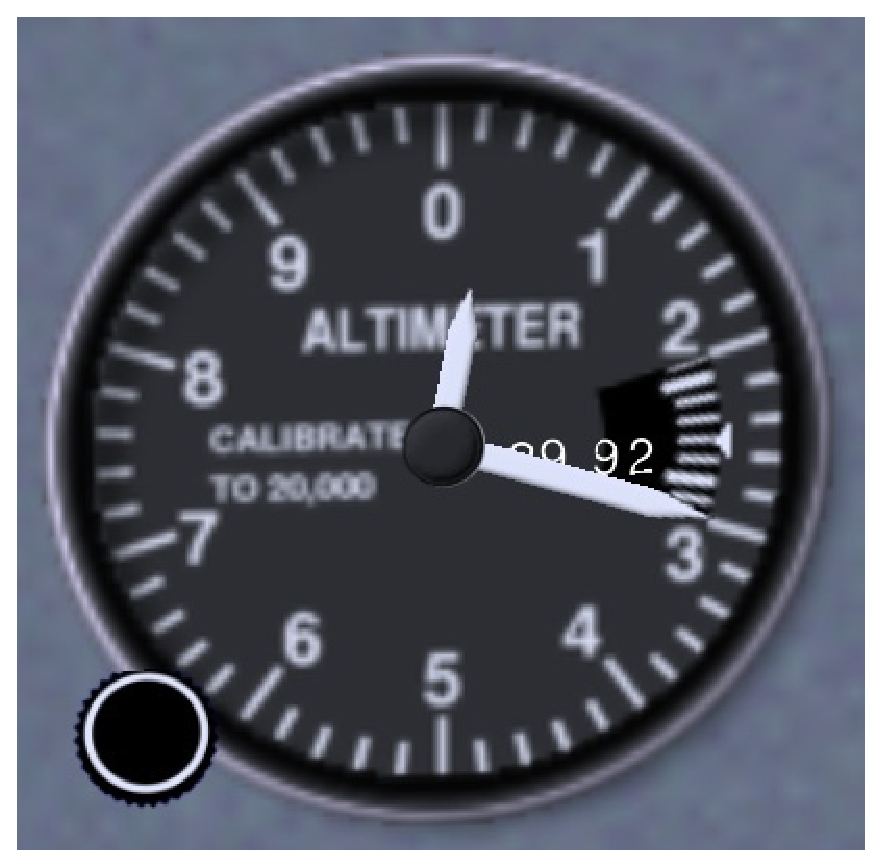
\includegraphics[width=0.25\textwidth]{img/tut_17}
\end{center}

As you ascend or descend the altimeter will change accordingly, turning
anti-clockwise as you descend, and clockwise as you gain height. If you see
the altimeter ``unwinding'' you will be able to tell that you are losing height
and move the mouse backwards slightly to raise the nose.
After a while you will notice that when flying level the nose of the aircraft
is always in the same position relative to the horizon. This is the aircraft
attitude for level flight. By putting the nose in that same position, you will
achieve almost level flight without having to reference the instruments. From
there you can fine-tune your altitude.

Beware: an altimeter does not automatically show the absolute altitude
above sea level\index{altitude!absolute}. You must adjust for the local air
pressive. The little black knob on the lower left side of the
altimeter\index{altimeter!tuning} allows you to adjust the altimeter. Start
\FlightGear{} and stay on the ground. Click (in normal mouse mode) inside the
black knob. A click on the left half makes the altimeter turn back. On the
right half the altimeter turns forward. Use that little knob to tune in the
current altitude. The principle is you use the knob when you are sure about
the altitude. If you know you are at 1,100 feet altitude, tune in 1,100 feet
on the altimeter. Clicking with the middle mouse button makes the knob
turn faster, or you can use the scrollwheel on your mouse.
Type \key{Ctrl}-\key{c} to see the two button halves highlighted.

To make settings the altimeter easier, airports advertise their altitude in
various ways. They may provide a radio service (called ATIS in the USA)
to broadcast the current air pressure at sea level. This is expressed in
inches of mercury. The altimeter contains a small scale inside which is
calibrated in this way. You can set your altimeter using this scale.
Alternatively, if you are on the ground and know the altitude of the airport,
you can simply adjust your altimeter until it displays the correct altitude.

\begin{center}
\includegraphics[width=0.25\textwidth]{img/tut_18}
\end{center}

Note that there is an important difference between ``altitude above sea
level'' and ``altitude above the ground''. If you fly near Mount Everest at an
altitude of 24,000 feet above sea level (AMSL), your altitude above the ground
(AGL) will be much less. Knowing the altitude of the ground around you is
obviously useful.

\section{Basic Turns}
\label{sec:InFlightTurning}

While if you had enough fuel you could return to the same airport by flying
straight head for thousands of miles, being able to change direction will
make your flying more enjoyable and useful.

Once you are able to fly more or less straight, it is time to
learn to turn. The principle is simple:
\begin{itemize}
    \item When the airplane is banked to the left, it turns to the left.
  \item When the airplane is banked to the right, it turns to the right.
\end{itemize}

\begin{center}
\includegraphics[width=0.25\textwidth]{img/tut_19}
\end{center}
\index{turn coordinator}

\index{turn coordinator} To turn, you do not need high levels of bank.
20$\textdegree$ is more than enough for a safe and steady turn. The turn
coordinator indicates your angle of bank by showing a depiction of your aircraft
from behind. The picture below shows the turn coordinator when the airplane is
banked 20$\textdegree$ to the right. You can also tell the bank angle by
observing the angle of the horizon.

Try the following: keep the airplane banked around those 20$\textdegree$ for a
few minutes and keep your eyes outside the aircraft You will see the same
ground features appear again and again, every 120 seconds. This shows you
need 120 seconds to make a 360$\textdegree$ turn (or 60 seconds for a
180$\textdegree$)turn). This is particularly useful when navigating.
Whatever speed the airplane is flying, if you bank at 20$\textdegree$ you
always need 60 seconds to make a 180$\textdegree$ turn in the Cessna 172P.

So, by banking the airplane to the left or to the right, you make it turn to
the left or to the right. Keeping the airplane level with the horizon keeps
it flying straight.

The little purple ball in the bottom of the turn indicator
shows the sideways forces. In real life you would feel these as your turn,
however it is not possible to simulate these, so you must simply keep an eye
on the ball. If you turn neatly (using the rudder a little bit),
the ball will remain centered. If the ball is pushed say rightwards, this
means you the pilot too are pushed rightwards. Like in a car turning to the
left. During a neat turn in an airplane, even a strong turn, the passengers
never endure a sideways force. They are only pushed a little harder on their
seats by the centrifugal force.

By experimenting you will notice you can make much steeper turns by
banking the airplane to high angles and pulling back on the yoke. Turns at over
60$\textdegree$ bank angle are the realm of aerobatics and military flying, and
dangerous is aircraft such as the Cessna.

\section{Taxiing on the ground}
\label{sec:TaxiTurning}

While \FlightGear{} starts you by default conveniently lined up on the
runway and ready to go, you may be wondering how to get your aircraft from
its hangar, along the taxi-ways to the runway. This is taxiing.

The picture below shows the \index{tachometer} instrument. It displays how fast
the engine is turning in hundreds of revolutions per minute (RPM).

\begin{center}
\includegraphics[width=0.25\textwidth]{img/tut_20}
\end{center}

Type the \key{Page Up} key a few times,
until the tachometer is showing 1,000 RPM (as shown above). If required
type the \key{Page Down} key to decrease the engine speed.

At roughly 1,000 RPM, the airplane will move forward on the runway, but it will
not accelerate and take off.

\index{brakes!right wheel [.] (dot)} Type the ``\key{.}''key (\key{Shift-;} on
Azerty keyboards). The airplane will make a sharp turn to the right. If you
keep the ``\key{.}''key down the airplane will halt. When you type the
``\key{.}'' key, you are activating the brake on the right wheel of the
airplane.

\index{brakes!left wheel [,] (colon)} To activate the brake on the left
wheel, use the ``\key{,}'' key.

\index{brakes} The ``\key{,}'' and ``\key{.}''  keys simulate two brake pedals
located at your feet on a real airplane. Using the throttle and the brake pedals
you can control the speed of the aircraft and cause it to turn on the ground.

The brakes can be very useful when taxiing slowly on the runway. You can also
steer the nose-wheel of the aircraft. In a real airplane this is done by pushing
the rudder pedals with your feet. You push with your feet on the side you want
to turn towards. If you don't have real rudder pedals, there are two ways to
control the virtual rudder pedals:
\begin{itemize}
    \item Using the keypad  \key{0} and \key{Enter} keys
  \index{rudder!keyboard control}. If you type the keypad \key{Enter} key say
  seven times, you will see the airplane firmly turns to the right and
  stays turning that way. Type the keypad \key{0} key seven times to get the
  airplane back rolling (almost) straight.
    \item Using the mouse. While the mouse is in yoke control mode
  ($+$ pointer shape), if you hold the left mouse button down, the mouse
  controls the rudder pedals instead of the yoke. The rudder pedals are
  connected to both the rudder \index{mouse!rudder control}
  \index{rudder!mouse control} and nose-wheel. This method is much more precise.
\end{itemize}

Start the simulator, Type \key{v} or \key{V} to view the airplane from
the outside and keep \key{x} down a couple of seconds to zoom in on the
airplane. Look at the front wheel and keep keypad \key{0} down. Then
keep keypad \key{Enter} down. See the front wheel turn. Press \key{Tab}
to get in yoke control mode ($+$ pointer shape).
Keep the left mouse button down to get in rudder control mode and move
the mouse to the left and to the right. Note that the rudder, that big
vertical control surface at the rear of the plane, moves together with
the front wheel.

I tend to control the rudder pedals using the mouse while the front
wheel is on the ground and use the keypad \key{0} and \key{Enter}
keys once it has lifted off. In other words: I
keep the left mouse button down while the front wheel is on the
ground. This allows for a precise and easy rudder control on the
ground. Then I simply release the left mouse button once the front wheel
lifts off.

\begin{center}
\includegraphics[width=0.5\textwidth]{img/tut_23}
\end{center}

\subsection{Airspeed}

Just like driving a car, it is good to know how fast you are traveling.
The aviation equivalent of a speedometer is the airspeed indicator (ASI),
calibrate in nautical miles per hour (knots).

\begin{center}
\includegraphics[width=0.25\textwidth]{img/tut_24}
\end{center}

A knot\index{speed!units!knot [nautical mile per hour]} is 1.85325
kilometer/hour. So, if you want to have a rough idea of your speed in
flight expressed in km/h, multiply the knots displayed by 2. A knot is
1.15115 miles per hour, so very roughly, 1 knot is 1 mph. Note that some
aircraft ASIs (in particular the Piper J3 Cub) display mph instead of knots.

The airspeed indicator displays the speed of the aircraft compared
to the surrounding air, not the speed compared to the ground like a car
speedometer does. If the plane is halted on the ground and there is
a 10 knot wind blowing from straight ahead, the airspeed indicator will
display 10 knots airspeed, although the plane will not be moving relative to
the ground.

When the airplane rolls over the runway at more than 40 knots, you must
prevent the front wheel from touching the ground. The nosewheel is not designed
for high speeds and in real life would shimmy and wear out.

During take off, once over 40 knots you can make the front wheel leave the ground by pulling back
gently on the control yoke. Don't turn sharply at high speed on the ground.
Doing so may cause the aircraft to tip over.

The picture below shows the front wheel slightly lifted. Don't overdo
this. Keep the airplane's white nose cover well below the horizon. You
just need to lift the plane's nose very slightly.

\begin{center}
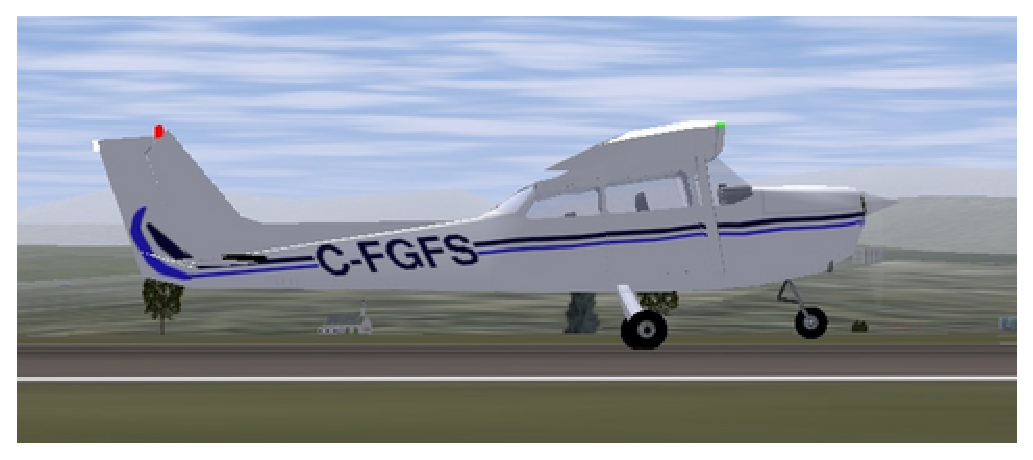
\includegraphics[width=0.5\textwidth]{img/tut_25}
\end{center}

Question: if the front wheel no longer touches the runway, how do you
steer the airplane? Answer: still using the rudder pedals. As mentioned above,
the rudder pedals are linked to both the nose-wheel and the tail rudder, that
big vertical moving part at the tail of the plane:

\begin{center}
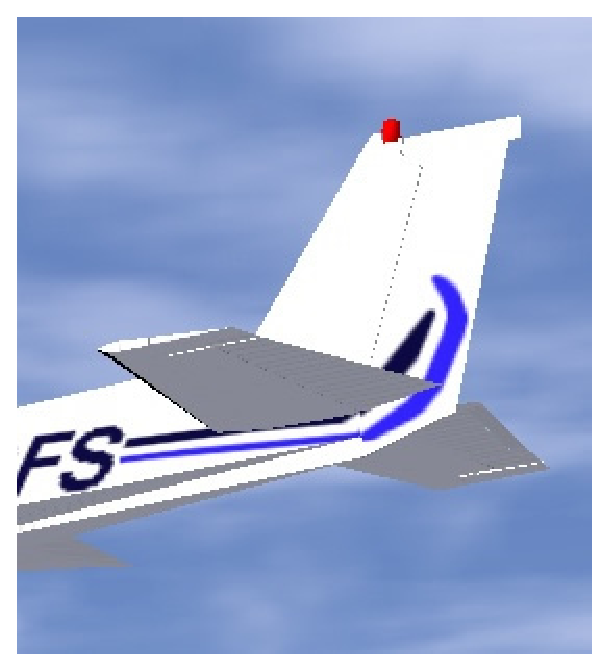
\includegraphics[width=0.5\textwidth]{img/tut_26}
\end{center}

At airspeeds above 40 knots, the rudder has enought air-flow over it to steer
the airplane.

Note the front wheel and the tail rudder don't make the airplane turn
at exactly the same rate. So when the rudder takes over the front wheel,
you must adapt the rudder pedals angle. That means fast typing keypad
\key{0} and keypad \key{Enter} (or hold the left mouse button down and
tightly control the rudder with the mouse).

Once you've become familiar with the nose-wheel and rudder, you can use these
new controls to keep the airplane straight on the runway during take-off.

Say the airplane is heading too much to the right. You type
keypad \key{0} a few times to make it turn back to the left. Don't
wait till the aircraft has straightened up completely. Type keypad \key{Enter}
before the aircraft reaches the direction you wish to travel. Otherwise you will
find that you will over-correct and have to turn back again. If you use the
mouse, such corrections are much easier and more precise.

To summarise: two methods exist to steer the airplane on the ground: the
differential brakes on the side wheels and the rudder pedals. This
control redundancy is very common in aviation. If one method fails,
you still have another method available to perform the task.

You may be wondering why the aircraft drifts to the left when it rolls on the
ground, forcing your to compensate with a little push on the right rudder
pedal? The main reason is the flow of air produced by the propeller. It
blows along the airplane body, but also corkscrews around the airplane
fuselage. The upper part of that slight vortex pushes the vertical tail
to the right. This causes makes the front of the aircraft to yaw to the left.

You can center all yoke and rudder controls by typing \key{5} on the
keypad. This is a good preflight precaution. Sometimes it can ``save
your life'' in flight if you find yourself with controls all over the place!

\section{Advanced Turns}
\label{sec:Turning}

As with turning on the ground, there are two methods of turning in the air.
You can use the wing ailerons (steered by the yoke/mouse) as described above or
you can use the tail rudder (steered by the rudder pedals / the
keypad keys /\key{0} and \key{Enter}.

Why two ways? Partially for redundancy, but mainly because they are
complementary. The main effect of the rudder is yaw (rotation around the
vertical axis), while the main effect of the ailerons is roll (rotation around
the longitudonal axis).

\begin{itemize}
    \item When flying close to the ground, it is better not to bank the
  airplane in order to turn. The rudder is used more instead. Acting on the
  rudder pedals allows you to turn the airplane without excessive banking.
    \item When the plane is just above the runway, the two side wheels need to
  be at the same height above the runway for landing. That means the wings
  must be level with the horizon. The plane is not allowed to bank. You keep
  the plane wings level with the horizon by using the yoke/mouse/ailerons.
  Note this does not need to be perfect. A bank of a few degrees is harmless.
    \item In flight, especially at high speed, the rudder is an in-efficient
  way to turn the aircraft:
\begin{itemize}
    \item It causes the airplane to present its flank to the airstream, increasing
  drag.
    \item The airplane turns very slowly.
    \item You will lack control while turning.
    \item At high flight speed the centrifugal force will be disturbing or even
  dangerous.
\end{itemize}
Using the yoke/mouse/ailerons allows for efficient, fast, reliable and
comfortable turns.
  \item The rudder can be vital when the wings are stalled. Indeed, during a
  stall the wing ailerons become less effective or even useless.
  (Note that some airplanes can go in a very dangerous stall if you overdo the
  rudder control at low speed.)
\end{itemize}

When you turn in flight, using the ailerons, you still need the rudder
a little bit. You add a little bit of rudder. This allows you to
compensate for the adverse yaw created when you roll using the
ailerons. In a real aircraft, you can feel this sideways motion. In the
simulator, you can check this visually on the turn coordinator. In the
picture below the little ball is pushed rightwards during a strong turn
to the right using the ailerons. That means you the pilot endure a rightwards
force too. You can compensate this by pushing the right rudder pedal
(type the keypad \key{Enter} key a few times). In normal flight you should use
the rudder to keep the little ball centered.

\begin{center}
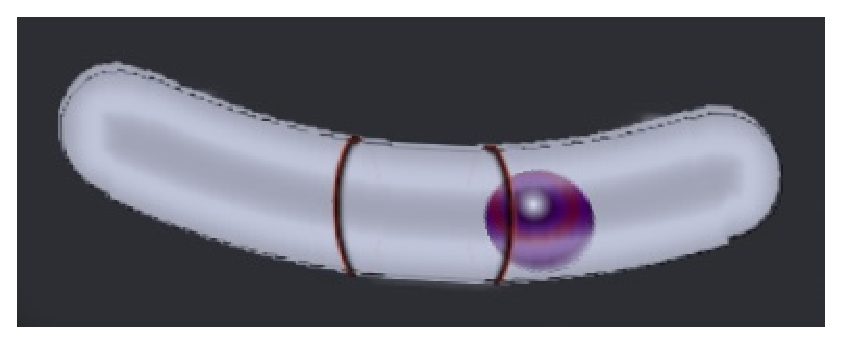
\includegraphics[width=0.25\textwidth]{img/tut_27}
\end{center}

So, in normal flight use the ailerons to turn, while close to the ground at low
speed use the rudder. However, one method never completely cancels out the
other. You still need the rudder at high altitudes and speeds. Reciprocally you
have to use the ailerons a little bit when close to the ground, to keep the
wings level with the horizon.

Even when taxiing, you should use the ailerons. Otherwise, strong winds can
blow the aircraft onto its side. To counteract this, your should turn the
ailerons into the wind. This raises the aileron in the wind, helping to
keep the wing down.

You should avoid making quick and agressive movements of the rudder. On the
ground at high speed this can make the airplane turn too sharply. In flight
at low speed it can cause a very dangerous type of stall. In flight at high
speed it can cause all kinds of aerodynamic and physical discomfort.
Instead, make gentle movements of the rudder.

I recommend you practise turning with the rudder in flight. Fly at a low
speed of about 70 knots. Try to keep the altitude stable by increasing
and decreasing the engine power. Use the rudder to turn towards a ground
feature and maintain a heading, then turn the aircraft towards a new heading.
See how the plane yaws. Learn to anticipate rudder
control. Don't try to make steep turns. Use the yoke/ailerons to keep
the wings level constantly.

\section{A Bit of Wieheisterology}

Wieheisterology comes from the German phrase ``Wie hei\ss t Er'' --
``What's that name''. This section is about gauges, switches and controls of
the aircraft. While in the simulator you can take off and land a basic airplane
with just the engine throttle and the yoke, but you will need all the controls to
perform securely and efficiently.

\subsection{Engine control}
\label{sec:EngineControl}

An airplane engine is designed for simplicity, reliability and efficiency.
Rather than use advanced electronic ignition and fuel injection systems found in
modern cars, they instead use older technology that doesn't rely on electrical
power. That way, the plane can still fly even if it suffers complete electrical
failure.

\subsection*{Magneto}\index{magneto}

On the bottom left, below the instrument panel you will find the
magneto switch and engine starter:


\begin{center}
\includegraphics[width=0.25\textwidth]{img/tut_28}
\end{center}

To see the switch, either type  \key{P} to get the schematic instrument
panel or type \key{Shift-x} to zoom out (\key{x} or \key{Ctrl-x} to
zoom back in).

You can move the switch with the \key{\{} and \key{\}} keys (use the \key{Alt
Gr} key on Azerty keyboards).

You are probably aware that the fuel inside a car engine is ignited by
electric sparks. Modern car engines use electronic ignition. An airplane engine
uses a more old-fashioned (but more reliable) magneto ignition instead. For
redundancy, it contains two such magnetos: the ``left'' one and the ``right''
one. When you change the magneto switch on OFF, both magnetos are switched off
and the engine will not run. With the magneto switch on L you are using the
left magneto. On R you are using the right magneto. On BOTH you use both.
In flight you will use BOTH.

Given that you use both magnetos in flight, why have the switch? The reason
is that during your pre-flight checks you will verify that each of the magnetos
is working correctly. To do this, increase the RPM to about 1500 then switch
the magneto switch to L and observe the tachometer. You should observe a
slight drop in RPM. If the engine cuts out, the left magneto is broken. If
you do not see an RPM drop, then the switch may be faulty, as both magnetos
are still switched on. You can then perform the same test on the right magneto.
Of course, in the simulator, the magnetos are unlikely to fail!

Should one of the two magnetos fail in flight, the other one will keep the
engine running. The failure of one magneto is rare, the failure of both
simultaneously is almost unheard of.

You may have typed \key{\{} to shut the engine down. To start
the engine again after doing so, type \key{\}} three
times in order to put the magneto switch on BOTH. Then use the starter motor
by pressing the \key{s} for a few seconds, till the engine is started.

You can also turn the magneto switch and start the engine by clicking
left and right of the switch in normal mouse mod). Type \key{Ctrl-c} to
see the two click sides highlighted by yellow rectangles.

If you turn the switch to OFF, the engine noise stops. If you quickly
turn the switch back to L, the engine starts again as the propeller is still
turning. If you wait for the propeller to stop, placing the switch on L, R
or BOTH won't start the engine. (Once the engine is halted, always place the
magneto switch to OFF.)

\subsection*{Throttle}\index{throttle lever}

\begin{center}
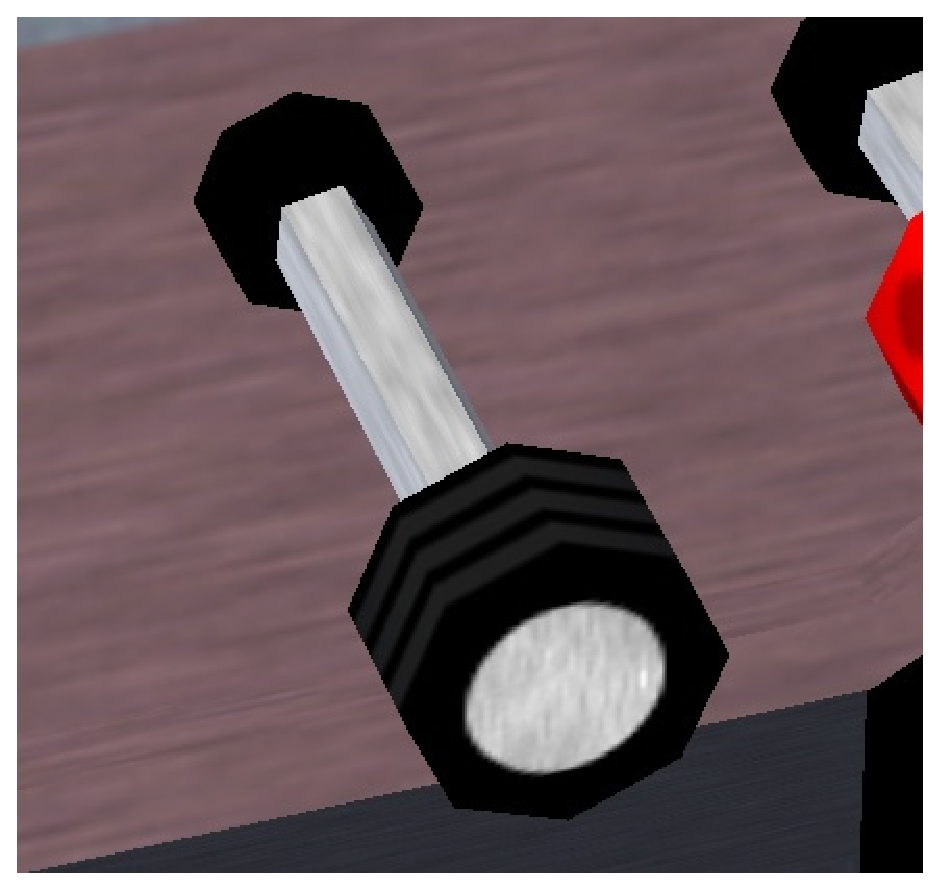
\includegraphics[width=0.25\textwidth]{img/tut_29}
\end{center}

You already know that you increase the engine power by pushing that throttle
rod in (\key{Page Up} key). You decrease the power by pulling the
control out (\key{Page Down} key). You can also click left and right of
the lever (middle mouse button for quicker moves, \key{Ctrl-c} to
highlight the left and right halves).

What does ``increase the power'' actually mean? Does it mean you increase
the amount of fuel delivered to the engine? Yes, but this is not enough to
fully understand what you are doing. You need to be aware that the engine is
also fed with a huge amount of air. The engine's cylinders burn an
\Index{mixture} of fuel and air. Fuel alone wouldn't burn.
Only a mixture of fuel and air can detonate and move the engine
pistons. So when you push the throttle in, you increase both the fuel
and the air fed to the engine.

\subsection*{Mixture}\index{mixture}

The amount of air compared to the amount of fuel is critical. The
proportion of the two has to be tuned closely. This is the purpose of
the mixture lever. The picture below displays the mixture lever, pulled out far
too much.

\begin{center}
\includegraphics[width=0.25\textwidth]{img/tut_30}
\end{center}

When the \index{mixture!lever} mixture lever is fully pushed in, you
feed the engine with an lots of fuel and little air. This is known as a
``rich'' mixture. When the lever is pulled out completely, there is an
excess of air, known as a ``lean'' mixture. The correct position to produce
maximum power is in between these two extremes, usually quite close to fully
pushed in.

When you start the engine and when you take off, you need a fuel-rich
mixture. That means the mixture lever should be pushed in. A fuel-rich mixture
allows the engine to start easily. It also makes the engine a little
more reliable. The drawback is that a part of the fuel is not burned
inside the engine. It is simply wasted and pushed out the exhaust. This makes
the engine more polluting, it decreases the energy the engine can deliver and
it slowly degrades the engine by causing deposits of residues inside the
cylinders.\index{mixture!optimisation}

Once in normal flight, you have to pull the mixture lever a little, to
get a more optimal mixture. Check this out by doing the following. Start
the simulator. Put the parking brakes on with key B (that is
\key{Shift-b}). Push the throttle in to its maximum. The engine RPM should
now be close to the maximum. Slowly pull on the mixture lever (using the
mouse in normal pointer mode). You will see the RPM increases a little.
You get more power, without increasing the fuel intake. You waste no
fuel and it pollutes less. If you continue to pull the mixture lever, the RPM
will decrease back away, because now there is too much air. The excess of air
slows the explosions down inside the cylinders and decreases the explosion
temperature, hence the thermodynamic yield decreases. You have to tune in the
optimal mixture. For thermodynamic reasons, the best mixture isn't exactly at
maximum power - it is better for the engine to be running very slight richer
or leaner than maximum power. This also avoids the possibility of the fuel
detonating explosively damaging the engine. You can find the
maximum power point by the fact you get the highest RPM. (Another method is to
check the engine exhaust temperature. Roughly, this is the point at which you
get the highest temperature.)

The mixture control allows you to burn less fuel for the same speed and
distance, and therefore fly farther and pollute less. However, if you
mis-manage it, it can cause serious problems.
Suppose you go flying at high altitude and pull out the
mixture lever accordingly. At high altitude there is less oxygen available
so the correct mixture will be quite lean - i.e. with little fuel being used.
Then you descend back in order to land. If you forget to push the mixture lever
in as you descend, The fuel/air mixture will become far too lean and the
engine will simply halt.

When landing, you have to tune back in a mixture that is a little too
rich in fuel. This means pushing the mixture lever in. That way the
engine becomes a little more reliable and will be better adapted to a
decrease in altitude.

I wrote above that placing the magneto on OFF is not the right way to
stop the engine. The right method is to pull the mixture
lever\index{engine!shut down}. First pull the throttle
out completely, to get the engine to minimum power and fuel
consumption. Then pull the mixture lever, till the engine stops because
the mixture contains too much air. This ensures the engine doesn't get
choked by waste fuel residues. Finally, turn the magneto switch to
OFF to ensure the engine won't start again accidentally.

An important warning: you may think the RPM indicator reflects the
engine power. Wrong. Two things make the RPM increase: the engine power
and the airplane speed. To check this, fly to a given altitude
then pull the engine power to minimum. Try out diving to the ground
then rising back to altitude. You will see the RPM varies significantly as does
your airspeed. It rises while diving and decreases while climbing.

One pitfall of this is when you intend to tune the engine power in for
landing. Suppose you're descending towards the airport,
flying fast. You know the ideal RPM for landing is around 1,900 RPM. So
you pull the throttle till you get 1,900 RPM. You think you tuned in
the appropriate RPM. You think you shouldn't bother any more about it.
But when you level off, the plane's speed starts to decrease, along with the
RPM. A few minutes later, you get the low flight speed you wanted. You don't
see the RPM is now far too slow. You will either lose altitude or
stall. Or both. Be cautious with the throttle and with the RPM
indicator. Either pull on the throttle more steadily or be mentally
prepared to push it back in quickly.

\subsection{Wings and speed}
\label{sec:WingsAndForce}

Say you are flying with full engine power. Dropping the nose a little makes you
lose altitude and raising the nose a little makes you gain altitude. You may
think this is quite straightforward. The plane travels in the direction it is
heading; the direction the propeller is heading. This is not the best way to
think about it.
This model would be fine for a rocket, but not for an airplane. A rocket is
lifted by its engine, while a plane is lifted by its wings.
That's a huge difference.

Get a big rigid square of cardboard, hold it horizontally in your hand
with your arm stretched out and make it do fast horizontal movements
while rotating your torso. When the cardboard moves flat through the
air, it experiences no lift force. If you twist your arm slightly to
give the cardboard a slight upward angle, you will feel it tends to
lift in the air. There is an upward force acting on the cardboard.
That's the way a wing holds a plane in the air. The wings have a slight
upward angle and lift the airplane. The more angle you give the
cardboard, the more lift force. (Till you give it too steep an angle.
Then you will rather feel a brake force. The cardboard is ``stalling''
(see below).)

\begin{center}
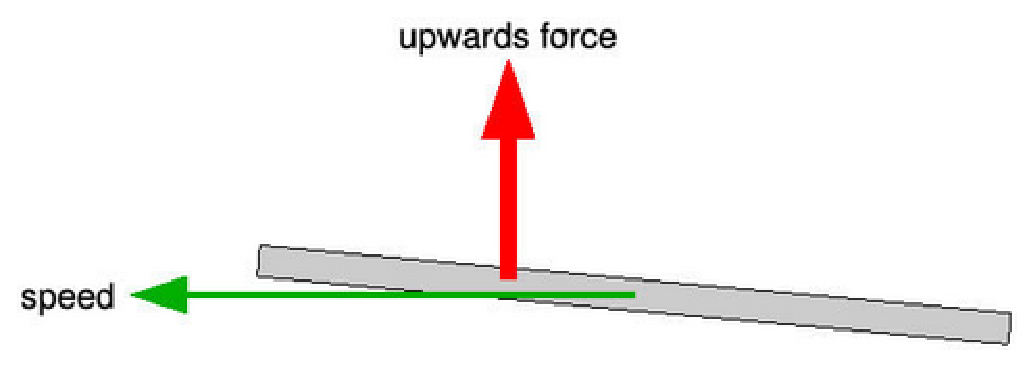
\includegraphics[width=0.5\textwidth]{img/tut_31}
\end{center}

\begin{itemize}
    \item When you pull the yoke, the airplane's nose rises up. Hence the wings
  travel through the air at a steeper angle. Hence the lift force on the
  wings is stronger. Hence the plane rises in the air.
  \item When you push the yoke, the airplane's nose dives. Hence the wings
  travel through the air with less angle. Hence the lift force on the wings
  decreases. Hence the plane descends.
\end{itemize}

What matters is the angle the wings travel through the air. This is the
angle of attack.

I wrote above that when the wings travel through the air with no angle of
attack, they don't produce lift. This is false. It would be true if the wings
were a flat plate like the cardboard. But they aren't. The wings are a
slightly curved airfoil. This makes them create lift even when traveling
through the air at no angle of attack. Actually, even with a little negative
angle of attack they still create a lift force. At high speed the airplane
flies with the wings slightly angled towards the ground!

\begin{center}
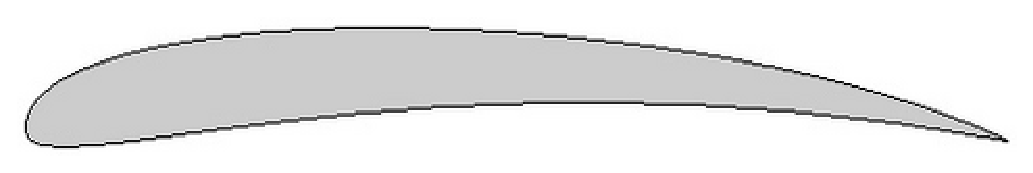
\includegraphics[width=0.5\textwidth]{img/tut_32}
\end{center}

The angle at which the wings travel through the air matters. Something
else matters too: the speed. Take the cardboard again in your hand.
Hold it with a given slight angle and don't change that angle. Move it at
different speeds through the air. The faster you move the cardboard, the more
upward force it experiences.
\begin{itemize}
    \item When you increase the engine power, the plane increases speed, the
  lift force on the wings increases and the plane gains altitude.
    \item When you decrease the engine power, the plane decreases speed, the
  lift force on the wings decreases and the plane loses altitude.
\end{itemize}

To make things a little more complicated: when rising in the air, the
airplane tends to lose speed. When descending, it tends to gain speed.

That's all a matter of compromises. If you want to fly at a constant
altitude and at a given speed, you will have to tune both the engine
power and the yoke/elevator (or better: the trim (see below)), till you
get what you want. If you want to descend yet keep the same speed, you
have to push the yoke a little and decrease the engine power. And so
on. You constantly have to tune both the engine power and the
yoke. However, during a normal flight you can simplify this by simply
choosing a comfortable engine power level then relying on the yoke and
trim for altitude.

A very interesting exercise you can perform with the simulator is to
fly straight with full engine power. Get maximum speed while keeping in
horizontal flight. Then decrease the engine power to minimum. Pull steadily
on the yoke to keep the plane at constant altitude.
The plane slows down steadily, meanwhile you have pull more and more on the
yoke to stay level. Since the speed decreases the lift from the wing
will decrease, but you compensate the loss of speed by increasing the wing
angle of attack. This proves the plane does not necessarily travel in the
direction its nose is heading. In this experiment we make the nose rise
in order to stay at constant altitude. Once the plane is flying very slowly,
and the nose is very high, you may hear a
siren yell. That's the stall warning (see below). This indicates that the angle
of attack is too high for the airfoil to produce lift. The wings are
no longer producing lift and the plane quickly loses
altitude. The only way to correct this is push the yoke forwards to reduce the
angle of attach, making the nose drop, then apply full power to gain speed and
finally bring the yoke carefully back to level flight.

Question: is it better to control the airplane's speed and altitude
with the yoke or with the throttle? Answer: it depends on what exactly
you intent to do and on the situation you are in. In normal flight, as
said above, you tend to set a comfortable engine power level, forget
about it and rely on the yoke and trim. During take off and landing the
procedures are quite strict about the use of yoke and throttle. You do
the opposite: control the speed with the yoke and trim, control the
altitude and descent speed with the engine throttle. This will be
discussed further below.

\subsection{The flaps} \index{flaps}
\label{sec:Flaps}

The flaps are situated at the rear of the wings, either side of the
aircraft fuselage.

\begin{center}
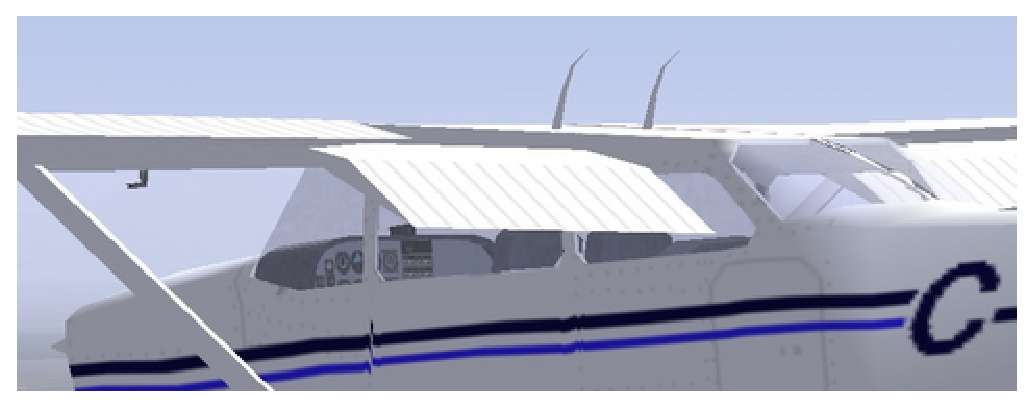
\includegraphics[width=0.5\textwidth]{img/tut_33}
\end{center}

You deploy the flaps and retract them back in by using the
\index{flaps!control lever}flaps control lever:


\begin{center}
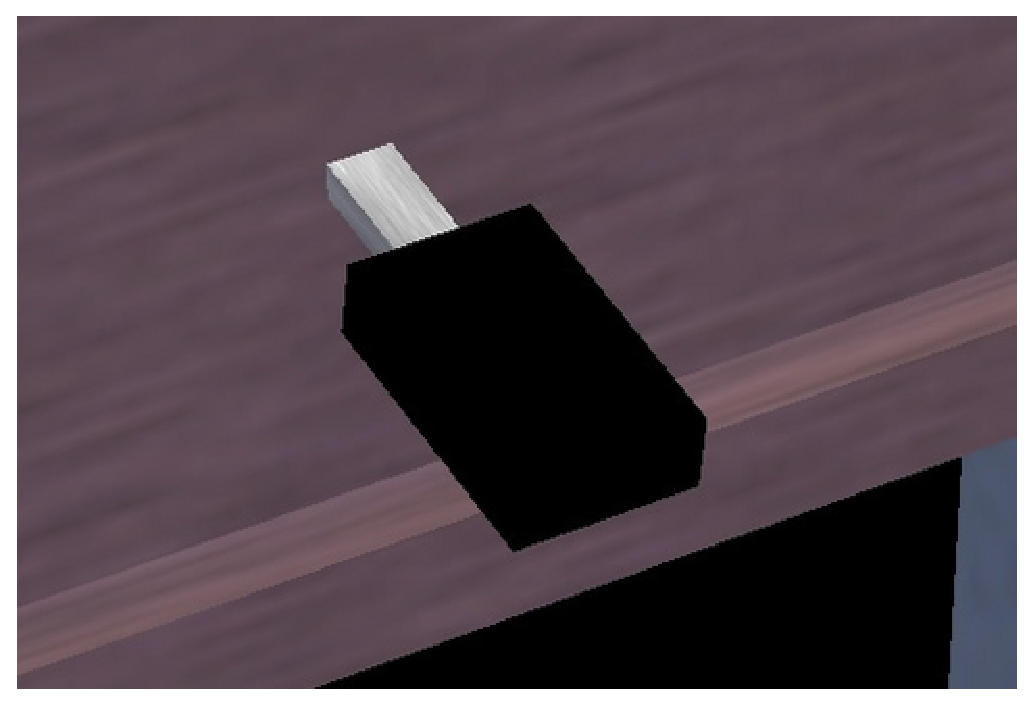
\includegraphics[width=0.25\textwidth]{img/tut_34}
\end{center}

You can either click on it with the mouse or use the \key{[} and
\key{]} keys. Key \key{[} to retract the flaps one step, \key{]} to
deploy them one step at a time. Type \key{v} to view the plane from the outside
and try out \key{[} and \key{]}. (On the schematic instrument panel the
flaps lever is located at the lower right.)

In the Cessna 172P. there are four \index{flaps!steps}flaps settings:
\begin{itemize}
    \item 0$\textdegree$ - for normal flight and normal take off.
    \item 10$\textdegree$ - for short field take off, when you want to gain altitude while
  flying slowly. Or during the first stange of an approach to land.
    \item 20$\textdegree$ - to slow the aircraft and lose altitude quickly, for example
  when descending towards the runway to land.
    \item 30$\textdegree$ - To lose altitude even more quickly.
\end{itemize}

The flaps are somewhat delicate. Do not deploy the first step of flaps above
110 knots. Do not deploy the second or third stage of flaps above 85 knots.

The flaps create large amounts of drag on the aircraft and brake the plane at
high speed. This is one more reason not to forget to pull the flaps back in
once you fly above 85 or 110 knots.

To check the flaps position visually, either use the mouse view mode to look
at the back of the wing, or type \key{Shift}-\key{right arrow} to shift the
view to the right and then quickly \key{Shift}-\key{up
arrow} to get back to front view.

Flaps increase wing lift by altering the shape of the airfoil. The wing lifts
more at a given speed with the first stage of flaps set. Hence you will get in
the air a little sooner during take off. It also has the effect to make the
plane fly with a lower nose attitude. This is useful as it provides a better
view of the runway when taking off or landing.

The flaps also increase drag on the aircraft. The second and third stage of
flaps produce much more drag than lift, so they are used to brake the
plane. This is particularly useful when landing, because the airplane glides
very well. If you cut down the engine power completely, the plane will descend, yet
but too slowly. You need to deploy two or three flaps steps in order to
brake and really descend towards the ground.

The fact that the flaps brake during landing makes you need more engine
power during the landing. This can seem odd. Why not simply throttle
the engine down to minimum and use less flaps steps? The answer is that it is
better to have a strongly braking plane and lots of engine power,
as the plane reacts faster to your commands. Should the
engine fail, then just retract flaps as needed and glide to the runway.

\index{side-slip}
What can you do if you have full flaps extended and need to increase your
rate of descent further? Slowly push the rudder pedals on one
side. This will make the plane present its flank to the air stream and
brake. Compensate the turning by using the ailerons (yoke). This is known as
side-slipping, and is a very effective way to lose height progressively as it
is easy to stop at any point.

\subsection{The stall}\index{stall}
\label{sec:Stall}

An aircraft relies on the smooth flow of air over the surface of the wing to
produce lift. However, if the wing is at too high an angle of attack, this
flow is broken, and the wing no-longer produces lift. With no lift, the
aircraft cannot fly, and quickly drops back to earth. This is known as a stall.

A stall is an emergency situation, whatever the While it can happen at any
speed, it commonly occurs in slow flight. A given aircraft has a specific
stall speed, at which no angle of attack can produce enough lift. You should
always keep your aircraft well above the stall speed. To help, aircraft
are equipped with stall sirens that sound when the angle of attack is
approached.

If you encounter a stall, the remedial action is to immediately
drop the nose, and apply full power, bringing the nose level when flying
speed has been attained again. However, doing so will cause the aircraft to lose
altitude, which you may not have to spare when landing or taking off!

\index{spin}A spin occurs when one wing stalls before the other, which can
occur in a steep turn at low speed. As one wing is still flying, the aircraft
turns around the stalled wing, spinning tighter and tighter. To get out of a
spin, you need to apply rudder to straighten out the spin into a normal stall,
then recover as above.

Aircraft like the Cessna 172 and Piper Cub, have benign stalls, and are unlikely
to enter a spin. High performance jets, such as the F16 have much more agressive
stalls, and can easily enter a spin.

To practise this in the simulator, do the following:
\begin{itemize}
    \item Fly at constant altitude and attitude.
  \item Reduce engine power, raising the nose to avoid entering a descent.
  \item Continue to reduce power until the stall begins.
  \item Try to control the plane while it stalls and descends to the ground.
  \item Keep the yoke pulled to the maximum and the plane in a steady attitude,
  the wings parallel with the horizon. Try to change direction.
  \item Recover by lowering the nose, applying full power, and correcting the
  attitude once flying speed has been regained.
\end{itemize}

You can also experiment with stalls with different flap settings, and high speed
stalls by making abrupt attitude changes.

Experiment with different aircraft. Compared with the Cessna 172 the Cessna
Citation jet, stalls much more agressively and with little warning..

\subsection{The trim}\index{trim}
\label{sec:Trim}

The trim is the dark big vertical wheel with gray dots located at the middle
below the instrument panel:

\begin{center}
\includegraphics[width=0.25\textwidth]{img/tut_35}
\end{center}

On \FlightGear, the keys \key{Home} and \key{End} adjust the trim.
\key{Home} rolls the wheel upwards while the \key{End} rolls the wheel
downwards. You can also click on the upper or lower half of the trim wheel.

In first approximation, the trim does the same as the yoke: it acts on
the elevator. Turning the trim wheel downwards is the same as pulling
on the yoke. Yet there is a key difference between the trim and the
yoke. The trim remains in position after you make a change, while the
yoke only continues to affect the elevator while you apply pressure and
returns the elevator to neutral when you release it.

During cruise flight, the required elevator position to keep the aircraft at
constand altitude will not be completely neutral - it will vary depending on
the air outside the aircraft, the current fuel level, and the payload.
Obviously, holding the yoke continually to retain a constant attitude would
quickly become tiring. By using the trim to ``trim out'' the elevator force
required for cruise flight, the yoke can be kept neutral.

During take off the trim should be neutral. Otherwise you may find that it
either refuses to take-off with the normal level of yoke control, or takes off
too quickly.

During landing, try to get the yoke/mouse/elevator towards neutral position
by tuning the trim. This makes making small adjustments to your attitude and
position easier. On the Cessna 172p this means trim on neutral. On the
Cherokee Warrior II this means the trim a little ``pulled''.

The trim wheel movement is much slower than the yoke, allowing for delicate
changes in trim. Be patient.


\subsection{What direction am I flying?}
\label{sec:Kierunek}

Knowing the direction you are going is obviously a good idea. There are three
basic ways to determine the direction you are flying:
\begin{itemize}
    \item Look through the windows. If you are flying regularly from the same
  airport, you will learn to recognize the ground features such as roads, hills,
  bridges, cities, forests. In a simulator, you only have a narrow view of the
  virtual outside world. Several ways exist to allow you to pan your virtual
  head inside the airplane:
      \begin{itemize}
        \item Use \key{Shift} and the four arrow keys to
      look to the front, rear, left and right.
        \item Use \key{Shift} and the keypad keys to look in the
      four directions mentioned above and in four diagonal directions
      in-between.
        \item Hold down the right mouse button in normal or yoke mode and move
        the  mouse to change the view direction.
        \item Use the mouse in view mode (\key{Tab}, $\leftrightarrow$). This
      allows you to look in every direction, including up and down. Click the
      left mouse button to bring the view back to straight ahead.
    \end{itemize}
 \item The magnetic compass. This is located above the instrument panel. The
 compass is simple, but is affected by the acceleration of the aircraft, and
 magnetic abnormalities on the ground. Also, the compass points towards magnetic
 north rather than true north. This deviation varies depending on your location.

\begin{center}
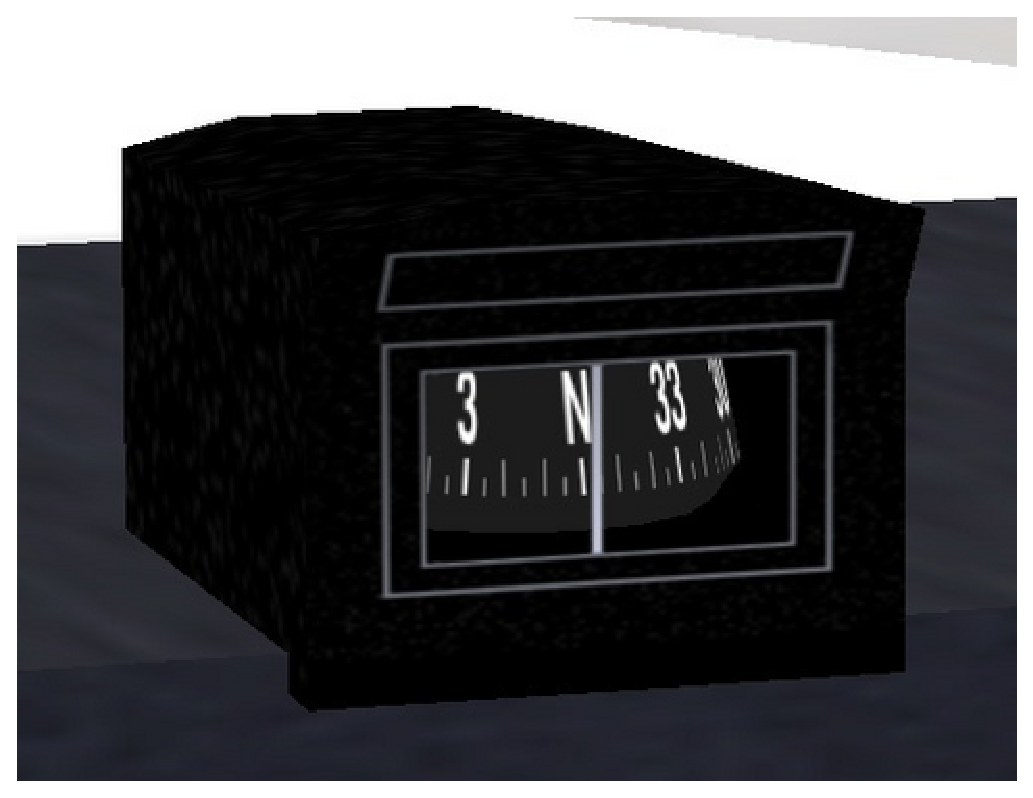
\includegraphics[width=0.25\textwidth]{img/tut_36}
\end{center}


  \item The directional gyro (picture below) or ``heading indicator''. The
  gyro is powered by a vacuum system. The gyro is set to match the magnetic
  compass, and is not affected by magnetic issues, or aircraft movement.
  However, due to gyroscopic precession and friction in the instrument, over
  time it drifts and must be reset by reference to the magnetic compass on
  ocassion. To reset the HI, during cruise flight, use the black knob on the
  bottom left of the instrument
  (normal mouse pointer mode, click left or right half of the knob, middle
  mouse button to move faster, \key{Ctrl}-\key{c} to highlight halves).
  (The red knob, bottom right, is used to tell the autopilot what direction
  you wish to fly (\textcolor{red}{\button{HDG}} = ``heading'').

\begin{center}
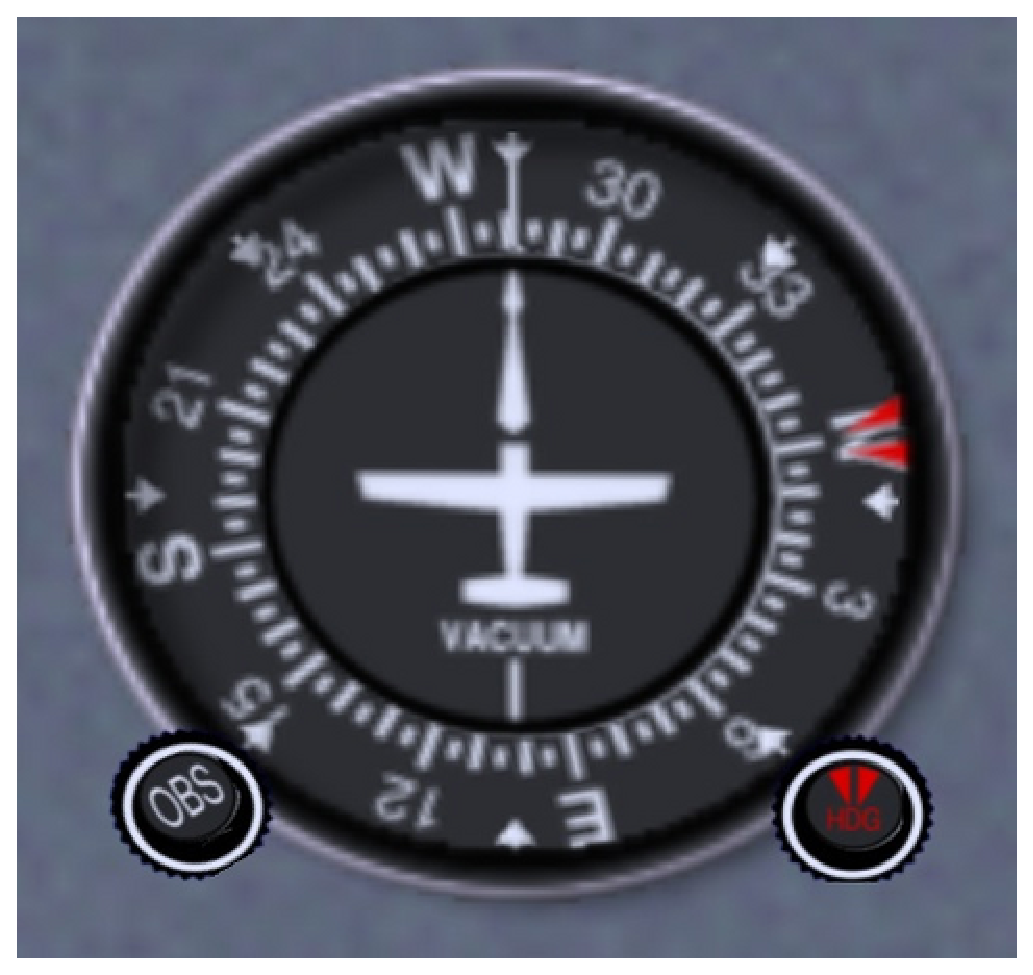
\includegraphics[width=0.25\textwidth]{img/tut_37}
\end{center}

\end{itemize}

\subsection{A look around the panel}

Finally, let's have a look at the instrument panel, combining the instruments
described above with some new ones.

\subsubsection{The six-pack}

Let us start with the most important instruments any simulator pilot must know,
these are known as the ``holy six'' or the ``six-pack''
.
In the center of the instrument panel (Fig.\,5), in the upper row, you will
find the \Index{artificial horizon} (\Index{attitude indicator}) displaying
\Index{pitch} and \Index{bank} of your plane. It has pitch marks as well as
bank marks at 10, 20, 30, 60, and 90 degrees.

Left of the artificial horizon, you'll see the \Index{airspeed indicator}. Not
only does it provide a speed indication in knots but also several arcs showing
characteristic \Index{velocity rages} you have to consider. At first, there is
a green arc indicating the normal operating range of speed with the \Index{flaps}
fully retracted. The white arc indicates the range of speed with flaps in action.
The yellow arc shows a range which should only be used in smooth air. The upper
end of it has a red radial indicating the speed you must never exceeded,
unless you want to break up the plane in mid-flights\ldots

Below the airspeed indicator you can find the \Index{turn indicator}. The
airplane in the middle indicates the roll of your plane. If the left or right
wing of the plane is aligned with one of the marks, this would indicate a
standard turn, i.e. a turn of 360 degrees in exactly two minutes.

Below the plane, still in the turn indicator, is the \Index{inclinometer}. It
indicates whether the \Index{rudder} and \Index{aileron}s are co-ordinated.
During turns, you always have to operate \Index{aileron} and \Index{rudder}
in such a way that the ball in the tube
remains centered; otherwise the plane is skidding. A simple rule says:
``Step on the ball'', i.e. step onto the left rudder pedal when
the ball is on the left-hand side.
\medskip

If you don't have pedals or lack the experience to handle the proper
ratio between aileron/rudder automatically, you can start \FlightGear{}
with the option \texttt{-$ $-enable-auto-coordination}.\index{auto
coordination}

To the right-hand side of the artificial horizon you will find the
\Index{altimeter} showing the height above sea level (not ground!) in hundreds
of feet.  Below the altimeter is the \Index{vertical speed indicator}
indicating the rate of climbing or sinking of your plane in hundreds of feet
per minute. While you may find it more convenient to use than the altimeter
in certain cases, keep in mind that its display usually has a certain time-lag.

Further below the vertical speed indicator is the propellor tachometer, or RPM
(rotations per minute) indicator\index{RPM indicator}, which displays the
rotations per minute in hundreds. The green arc marks the optimum region for
cruise flight.

The group of the main instruments further includes the \Index{gyro compass}
being situated below the artificial horizon. Besides this one, there is a
\Index{magnetic compass} sitting on top of the panel.

Four of these gauges being arranged in the from of a ``T'' are of special
importance: The air speed indicator, the artificial horizon, the altimeter,
and the compass should be scanned regularly during flight.

\subsubsection{Supplementary Instruments}

Beside the six-pack, there are several supplementary instruments. To the very
left you will find the \Index{clock}, obviously being an important tool
for instance for determining turn rates. Below the clock there are
several smaller gauges displaying the technical state of your engine.
Certainly the most important of them is the \Index{fuel indicator} - as
any pilot should know.

The \Index{ignition switch} is situated in the lower left corner of the
panel (cf. Fig.\,4). It has five positions: ``OFF'', ``L'', ``R'',
``BOTH'', and ``START''. The first one is obvious. ``L'' and ``R'' do
not refer to two engines (as the Cessna 172 only has one) but the
two magnetos, providing redundancy in the case of a failure.. The two switch
positions can be used for test puposes during preflight. During normal
flight the switch should point on ``BOTH''. The extreme right position
is for \index{starting the engine} using a battery-powered
\Index{starter} (operated with the ``s'' key).

The handle below the yoke is the parking brake. In the vertical position,
the parking brake is ON. The parking brake is operated with the ``B'' key.

\subsubsection{Radios}

The right hand side of the panel is occupied by the \Index{radio stack}. Here
you find two \Index{VOR} receivers (NAV),\index{NAV} an \Index{NDB} receiver
(\Index{ADF}) and two \Index{communication radio}s (COMM1/2)
\index{COMM1}\index{COMM2} as well as the autopilot.

The \Index{communication radio} is used for communication with \Index{air
traffic facilities}; it is just a usual radio transceiver working in a special
frequency range. The frequency is displayed in the LEDs. Usually
there are two \Index{COM transceiver}s; this way you can dial in the frequency
of the next controller to contact while still being in contact with the previous
one.

The COM radio can be used to listen to the current weather conditions at an
airport, known as ATIS. To do this, simply dial in the ATIS frequency of the
relevant airport. You can find this by selecting \texttt{ATC/AI->Frequencies}
from the menu, and selecting the 4-letter ICAO code of a nearby airport.

Each COM radio has two frequencies configured - an `active' frequency which
the pilot is transmitting and receiving on, and a `standby' frequency which may
be changed. In this way, you can continue to listen on one frequency while tuning
another one.

You can change the radio frequency using the mouse. For this
purpose, click left/right to the circular knob below the corresponding
number. The corresponding switch left to this knob can be used for
toggling between the active/standby frequency.

Use of the autopilot and radio navigation equipement is covered in later
tutorials. For the moment you can ignore these radio instruments as
long as you are strictly flying according to \Index{VFR} (\Index{visual
flight rules}).

\section{Let's Fly}

By now you will be able to keep on runway while
taking off by using the rudder and you're able to fly straight, descend, climb
and make gentle turns. This section will describe a slightly more realistic
approach to taking off and landing, and introduce some of the more subtle
concepts you should be aware of.

\subsection{A realistic take off}
\label{sec:Start}


The following general rules apply during a normal take-off:
\begin{itemize}
    \item The nose-wheel should be lifted from the runway at approximately 40
  knots.
  \item Immediately after take-off, you should accelerate to 70 knots, to stay
  well above stall speed, in case of a gust of wind, or engine failure.
  \item Don't fly much above 75 knots to ensure you gain height as quickly as
  possible.
  \item Follow the runway heading until at 500 feet. This way, if you suffer
  an engine failure, you can easily land back on the runway you left.
  \item Don't over-fly buildings until at least 1,000 ft.
    \item Close to the ground, turns should be gentle and well coordinated
  using the rudder.
\end{itemize}

So, you need to take off and rise in the air at a steady speed of around
75 knots. However, when you raise the nose slightly at 40 knots, the aircraft
will probably take-off at around 55 knots. To accelerate quickly to 75 knots,
lower the nose slightly immediately on take-off, then raise it once 75 knots
has been achieved. You are using the yoke to control the speed of the aircraft.

Putting this all together with what you have learned previously, a normal
take-off using the mouse will consist of the following:

\begin{enumerate}
  \item Adjust the altimeter to the correct altitude, based on the airport
  altitude. For reference, KSFO is at sea level - 0ft.
    \item Check aileron and elevator are neutral by observing the yoke position.
  \item Change the mouse to control mode by pressing \key{Tab}.
  \item Hold the left mouse button down to control the rudder.
  \item Apply full power (hold \key{PgUp} until the throttle is fully in).
  \item As the aircraft accelerates down the runway, keep it in the center by
  making small adjustments using the mouse.
  \item As 40kts is reached, release the left mouse button, and pull back
  slightly to raise the nose-wheel. You are now controlling the yoke with the
  mouse.
  \item The aircraft will fly off the runway at approximately 55 knots.
  \item Lower the nose slightly to accelerate to 70 knots
  \item Keep alignment with the runway.
  \item Use the yoke to keep the ASI at 70 knots as you climb. If the airspeed
  is dropping, lower the nose. If the airspeed is increasing, raise the nose
  slightly.
  \item Once you reach 500 feet, turn to your required heading, staying away from
  buildings until you are over 1,000ft.
\end{enumerate}

\subsection{Landing}\index{landing}
\label{sec:Ladowanie}

The rules for landing are almost identical to that of take-off, but in reverse
order:
\begin{itemize}
    \item Close to the ground, turns should be gentle and well coordinated
  using the rudder.
  \item Stay above 500ft until on final approach to the runway
    \item Approach the runway at approximately 70 knots.
    \item Touch down on the two main wheels at 55kts.
  \item Let the nosewheel touch down at 40kts.
\end{itemize}

Landings are much easier if you have an aiming point picked out on the runway.
By observing the aiming point, you can easily tell if you are descending too
fast or too slowly. If the aiming point appears to move upwards, you are
descending too fast,

Obviously, you need to be lined up with the runway.That means your flight
direction has to match the middle line of the runway (drawing (a)
below). In order to arrive at this, don't aim at the start of the
runway (b). Rather aim at a fictitious point well in front of the runway
(c). And begin to turn gently towards the runway well before you reach
that fictitious point (d). Note the turns and bankings you make for
these flight corrections are often very soft. You wouldn't even notice
them on the turn coordinator. This is one example where you better rely
on the outside horizon line than on the inside flight instruments.

\begin{center}
\includegraphics[width=1.0\textwidth]{img/tut_41}
\end{center}

A straight in landing using the mouse would consist of the following:
\begin{enumerate}
  \item 1,500ft above the airport, and a couple of miles out, an in-line with
  the runway, reduce power to approximately 1500rpm. This will slow you down
  somewhat and start a gradual descent.
  \item Once below 115 knots, apply one step of flaps (\key{]}). This will
  increase lift, but also slow you down.
  \item Re-trim the aircraft so you continue to descend.
  \item At around 1,000 feet, apply another step of flaps (\key{]}). This
  increase drag significantly, but also improve the view over the nose.
    \item Tune the speed using the elevator and trim: push the yoke if you are
  flying below 70 knots, pull the yoke if you are flying above 70 knots. If
  using a joystick, use the trim to relieve any pressure on the elevator.
  \item Tune the altitude using the engine throttle. Add power if you are
  descending too fast, reduce power if you are too high. It is much easier to
  work out if you are too high or too low by observing the numbers on the runway.
  If they are moving up the screen, you are descending too fast - increase power.
  If they are moving down, you are too high and need to reduce power.
  \item Make minor adjustments to heading to keep aligned with the runway.
  \item at about 500ft, apply the final step of flaps. (\key{]}). This
  increase drag significantly, so be prepared to increase power to keep your
  descent constant.
  \item When you are just above the runway, reduce power to idle, and use the
  yoke to gently pull back the aircraft to horizontal. This is the ``round-out''
  and should result in the aircraft flying level with the runway a couple of
  feet above the surface. Performing the round-out at the correct height is a
  difficult task to master. To make it easier, observe the horizon rather than
  getting fixated on the aiming point.
  \item Keep the wings level using small inputs with the yoke. We want both
  wheels to touch down at the same time.
  \item Continue pulling back on the yoke. The main wheels should touch down at
  about 55 knots. This is the ``flare''.
  \item As you touch down, be ready to use the rudder to keep the aircraft
  straight (keypad \key{0} and keypad \key{Enter})
  \item Once you are below 40 knots, lower the nose-wheel to the ground.
  \item Hold down the left mouse button to control the nosewheel/rudder using
  the mouse.
  \item Once below 30 knots, use the brakes \key{b} to slow the aircraft
  further.
\end{enumerate}

\begin{center}
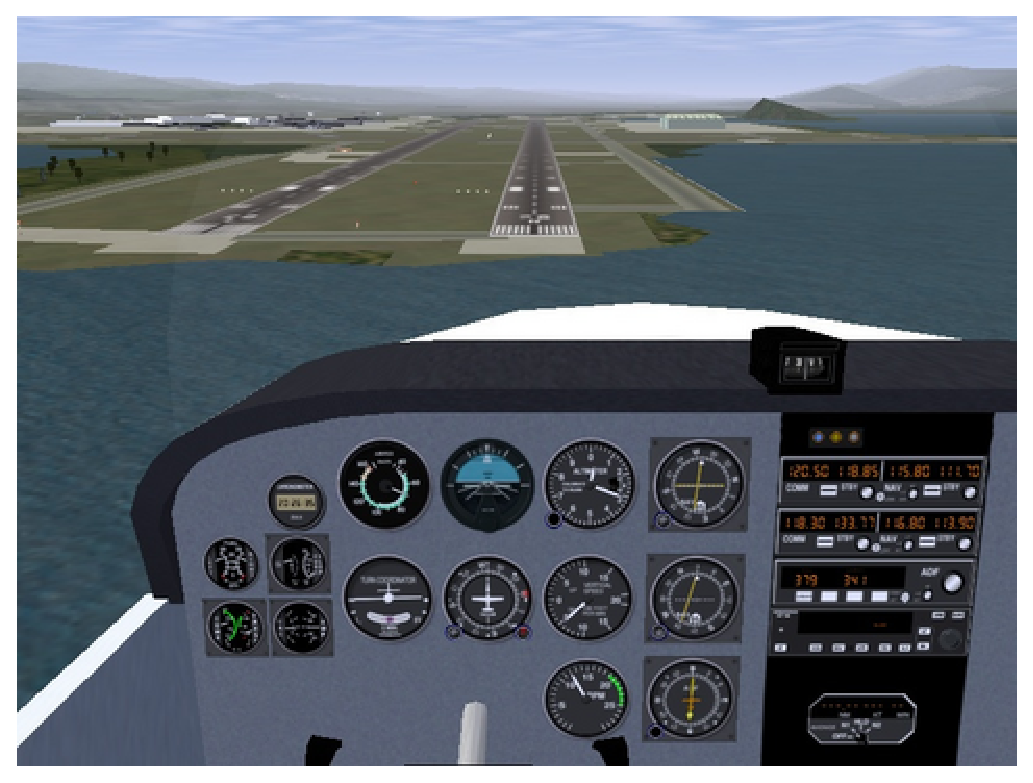
\includegraphics[width=0.5\textwidth]{img/tut_43}
\end{center}

Once the plane is halted or at very low speed, you can release the \key{b} key
and add a little engine power to taxi to the parking or hangar.

\subsection{Engine Shutdown}\index{shutdown}

To shut the engine down:
\begin{itemize}
  \item Set the parking brake, type \key{B}.
    \item Engine throttle to minimum (hold \key{Page Down} down for a while).
    \item Pull the mixture lever to halt the engine (mouse in normal pointer mode,
  click on the left of the red mixture lever to pull it out).
  \item Rotate the magneto switch to OFF (a few hits on \key{\{}).
\end{itemize}

\subsection{Aborted Landing}\index{abort}

You must be mentally prepared to abort landing any time the landing doesn't look
good, or due to external factors such as:
\begin{itemize}
  \item an order from the control tower
  \item incorrect speed or landing angle when there is insufficient time to
  correct it.
  \item a strong gust blow of wind
  \item birds flying over the runway.
\end{itemize}

To abort the landing, apply full power (hold \key{PgUp}), raise the nose to climb,
and once you are climbing, retract the flaps (key{[}).

Landing is much harder than taking off. Landing on a large runway, such as KSFO
(San Francisco, the default) is much easier than smaller runways such as KHAF
(Half Moon Bay, about 10 miles to the south west of KSFO).

To practise landings, use the command line below in a terminal window to start
the simulator in flight and heading for the runway. The airplane is placed 5
miles ahead of the runway, at an altitude of \textbf{1500} feet and a speed of
about 120 knots.

\command{fgfs -$ $-offset-distance=5 -$ $-altitude=1500 -$ $-vc=120 -$ $-timeofday=noon}

Approaching to land at 65 knots instead of 70 knots allows to use a much shorter runway
length. However, this requires better control, particularly as it is much closer
to the stall speed. It is quite different from landing at 70 knots.

\section{Dealing with the Wind}
\label{sec:Fwsw}

Consider a hot air balloon. Think of it as being in the middle of a gigantic
cube of air. The cube of air may move at high speed compared to the ground,
but the balloon itself is completely static in the middle of the cube. Whatever
the wind speed, persons aboard a hot air balloon experience not a breath of
wind.

In the same way, an aircraft flies in the middle of a gigantic cube of air
and flies relative to that air mass. The motion of the cube of air
relative to the ground has no effect on the aircraft.

You, the pilot, on the contrary, are interested in the speed of the
surrounding air compared to the ground. It can make you drift to the
left or to the right. It can make you arrive at your destination much
later or much sooner than planed.

When the wind blows in the same direction as you fly, the speed of the
wind adds itself to the airspeed of the plane. Hence you move faster
compared to the ground. You will arrive earlier at your destination.

When the wind blows in the opposite direction (towards the nose
of the plane), the speed of the wind subtracts itself from the airspeed
of the plane. Hence you move slower compared to the ground. You will
arrive later at your destination and have more time to enjoy the
landscape.

The two cases above are quite simple. More complex is when the wind blows
towards the side of the airplane. Consider the diagram below.

\begin{itemize}
    \item On picture (a) there is no wind. The pilot wants to reach the green
  hill situated to the North. He heads for the hill, towards the North, and
  reaches the hill after a while. When there is no wind, you just head towards
  your destination and everything's fine.
    \item On picture (b), the pilot keeps heading to the North. Yet there is wind
  blowing from the left; from the West. The airplane drifts to the right and
  misses the hill.
    \item On picture (c), the pilot keeps heading towards the hill. This time he
  will arrive at the hill. Yet the plane flies a curved path. This makes the
  pilot lose time to get to the hill. Such a curved path is awful when you need
  to make precise navigation.
    \item Picture (d) shows the optimal way to get to the hill. The plane is
  directed to the left of the hill, slightly towards the West and the wind.
  That way it compensates for the wind and remains on a straight path towards
  the hill.
\end{itemize}

\begin{center}
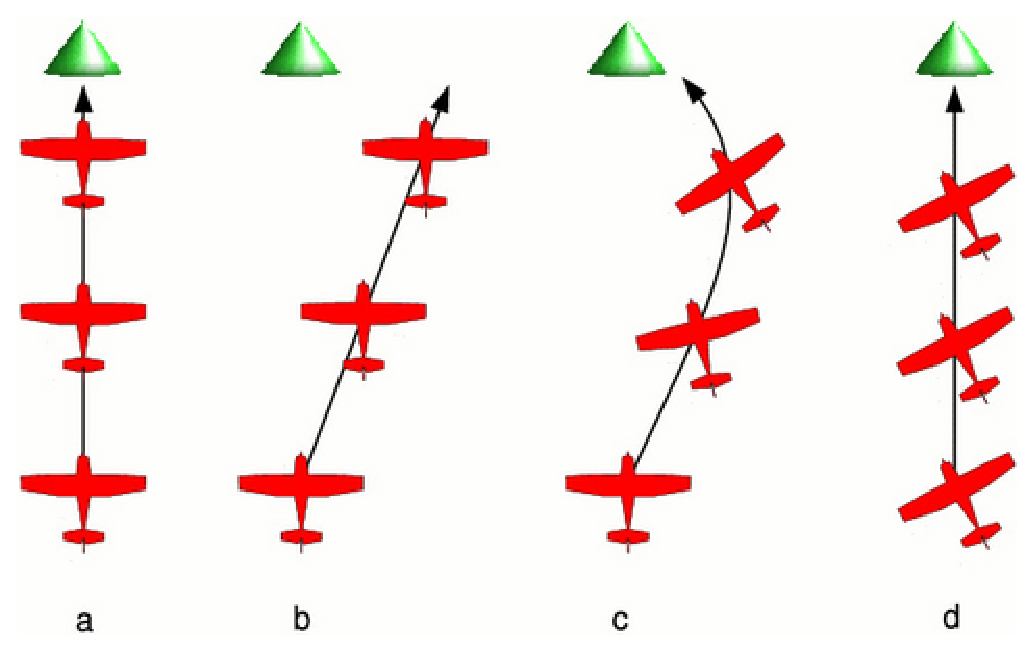
\includegraphics[width=1.0\textwidth]{img/tut_44}
\end{center}

How much to the left or to the right of the object must you head? At
what angle? Serious pilots use geometry and trigonometric
computations to calculate the correct angle. You need no
computations at all to fly roughly straight. The trick is to choose an aiming
point in the direction you wish to fly, then observe how it moves.
You will become aware if you are drifting leftwards or rightwards. Then let
your instinct slowly head the plane to the right or to the left to compensate
the obvious drift. To begin with, you may need to think about what you are
doing. Very soon this will become automatic, just like when you learned to fly
straight. You will no more keep the plane headed towards the object. You will
rather keep it flying towards the object.

The faster the flight airspeed compared to the wind speed, the less correction
you will need.

\subsection{Crosswind Take Off}
\label{sec:Swsw}

Taking off when the wind is coming from the side is tricky. Airport designers
avoid this by placing runways so that they face into the prevailing wind. Often
airports have multiple runways, placed such that there will be a runway facing
straight into wind as much of the time as possible.

Taking off with a wind blowing straight towards the nose of the aircraft makes
life easier as it is the speed of the wing relative to the air that causes
lift. When there is no wind, the aircraft must accelerate to 55 knots
to take off. However, if there is a 10 knot head-wind, the aircraft has an
airspeed of 10 knots standing still and only has to accelerate to 45 knots
relative to the ground to take off. This shortens take-off distances.

Just as a headwind shortens take-off, a tail-wind increases take-off length.
Anything more than a knot or two makes a huge difference to take-off distance.
As (most) runways can be flown from either end, you can easily take off from
the other end of the runway and benefit from the headwing.

The main way to know the wind direction and speed is to go to the
control tower or ask the control tower by radio. A necessary and
complementary tool are the windsocks\index{windsock}
at both ends of the runway. They show the wind direction and speed. The
longer and the stiffer the windsock, the more wind there is. The
windsock on the picture below shows an airspeed of 5 knots:

\begin{center}
\includegraphics[width=0.5\textwidth]{img/tut_46}
\end{center}


Unfortunately, sometimes there isn't a runway facing the wind, and you have to
take off when the wind is blowing from the side.

The technique is as for a normal take-off with two changes:
\begin{itemize}
    \item During the take-off roll, the aircraft will try to ``weather-cock'' into
  wind. You must react by using the rudder to keep the aircraft running
  straight. You will have to apply the rudder at quite a strong angle to stay
  aligned with the runway. You will need to keep applying rudder throughout
  the take-off.
  \item As you take off, the aircraft will react to the rudder and try to turn.
  You will need to correct for this using the ailerons. Once the aircraft is in
  the air, you can reduce the rudder pressure and aileron, then correct for
  the wind, to keep aligned with the runway as described above.
\end{itemize}

\subsection{Crosswind Landing}
\label{sec:Lwsw}

Landing in a crosswind is very similar to the take-off:
\begin{itemize}
    \item Stay aligned with the runway by compensating for the crosswind.
  \item As you begin to round-out, use the yoke to straighten the aircraft so
  it is pointed down the runway. Apply rudder to stop the aircraft turning.
  \item The aircraft will land on one wheel first. Use the rudder to keep the
  aircraft pointed straight down the runway as the other wheel touches down.
\end{itemize}

The technique described here is the
\weblong{http://en.wikipedia.org/wiki/Slip_landing}{slip landing}.
Another crosswind landing technique is the
\weblong{http://en.wikipedia.org/wiki/Crab_landing}{crab landing}.

\subsection{Taxiing in the Wind}
\label{sec:Twsw}

Under 10 knots wind the Cessna 172p seems not to need particular precautions
when taxiing. Yet any sudden increase in wind speed can tilt it and tumble
it over. So best apply the recommendations whenever there is wind.

To train taxiing on the ground when there is wind, configure the simulator for
a strong wind, like 20 knots. Such a wind can tilt the plane and blow it away
tumbling any moment. One single error during taxiing and the plane is lost.

Main rule is you must \emph{push the yoke towards the wind}. This deserves some
physical explanation:
\begin{itemize}
    \item When the wind is blowing from 12 o'clock, this is quite logical. The
  yoke is pushed (towards 12 o'clock) and the elevator makes the tail rise a
  little. That's the most stable position to avoid the plane be tilted by the
  wind.
    \item When the wind comes from 10 o'clock, pushing the yoke towards
  10 o'clock means that the elevator is almost neutral, while the
  left aileron is upward and the right aileron is downward. This pushes the
  left wing down and lifts the right wing. Again, that's the most stable
  position to avoid the plane be tilted by the wind.
  \item When the wind blows from 8 o'clock, you would think you should invert
  the position of the ailerons, to keep the left wing being pushed down. Hence
  you should push the yoke to 4 o'clock. Wrong! Keep pushing the yoke to 8
  o'clock. The reason is the downward position of the aileron on the right
  wing makes it act like a slat. This increases the lift on the right wing and
  this is all we want. Symmetrically, the upward position of the left aileron
  decreases the lift of the left wing.
  \item When the wind comes from the rear, from 6 o'clock, the yoke is
  pulled (towards 6 o'clock). The upward position of the elevator tends to
  make the tail be pushed down. Once again this is the best. Strong wind can
  push the tail against the ground. This is impressive but the tail is
  conceived to withstand this.
\end{itemize}

If you want to move towards the wind, you will need more engine power.
When the wind blows from the rear you may need no engine power at all.
Always keep the engine power to the minimum needed.

Especially when turning, move very slowly. Make little changes at a
time. Take your time and closely survey the yoke angle. Constantly keep
it pushed towards the wind. Constantly try to reduce the engine power.
Keep in mind using the brakes too firmly may shortly tilt the plane at
an angle that allows the wind to tilt it and blow it away.

\section{The autopilot}\index{autopilot}
\label{sec:Autopilot}

An autopilot is not an ``intelligent'' pilot. It just takes over simple tasks
for the pilot. You still are the pilot aboard and have to keep aware of
everything. Be prepared to shut the autopilot down as they often go wrong,
both in real life, and in the simulator.

The autopilot is mounted to the right of the yoke:

\begin{center}
\includegraphics[width=0.5\textwidth]{img/tut_49}
\end{center}

Switch it on by pressing the \button{AP} button.
The autopilot then controls the \index{autopilot!modes!roll control
mode}roll of the aircraft. It keeps the wings level with the horizon. This is
displayed in the picture below by the ``\textcolor{orange}{\button{ROL}}''
marking. To switch the autopilot off press \button{AP} again.

\begin{center}
\includegraphics[width=0.5\textwidth]{img/tut_50}
\end{center}

\index{autopilot!modes!heading mode} If you press the \button{HDG} button the autopilot will try to keep
the plane flying towards the direction tuned on the directional gyro by
the red marking (see section \ref{sec:Kierunek}).
``\textcolor{orange}{\button{HDG}}'' stands for ``heading''. Press
again on the \button{HDG} button to get back to roll control mode (or
\button{AP} to switch the autopilot off).

\begin{center}
\includegraphics[width=0.5\textwidth]{img/tut_51}
\end{center}

The buttons \button{ALT}, \button{UP} and \button{DN} are used to tell
the autopilot either to control the vertical
\index{autopilot!modes!vertical speed mode}speed
\textcolor{orange}{\button{VS}} or the altitude
\textcolor{orange}{\button{ALT}}.
For more advanced use of the autopilot, see the reference document for the
autopilot modelled in the Cessna 172:
\weblong{https://dealer.bendixking.com/servlet/com.honeywell.aes.utility.PDFDownLoadServlet?FileName=/TechPubs/repository/006-18034-0000_3.pdf}{Bendix King website}
\section{What Next?}
\label{sec:Poslowie}

This tutorial has introduced you to the basics fo flight in the Cessna 172. From
here you can explore the many features that \FlightGear{} has to offer.

Once you have mastered the content of this tutorial, you may want to look at the
other tutorials in this Manual, covering flying to other airports, flying using
instruments when clouds obscure the ground, and flying helicopters.

This tutorial has skipped over a number of topics that a real-life pilot would
have to consider:
\begin{itemize}
    \item How to follow real checklists.
    \item How to make emergency landing on very short fields, after and engine
  failure.
    \item How to navigate with regard to the laws of the air, charts, laws, radio
  beacons and weather conditions
    \item How to create a flight plan and fly it accurately.
    \item How to place people, fuel and baggage in an airplane to get a correct
  center of gravity.
    \item How to deal with the control tower and with other airplanes.
    \item How to deal with several fuel tanks and their systems.
    \item How to deal with the failure of every possible part of the plane.
\end{itemize}

This tutorial has also not covered features of more advanced aircraft,
including:
\begin{itemize}
  \item retractable landing gear
  \item variable pitch propellers
  \item multiple engines
  \item jet engines.
\end{itemize}

\section{Thanks}

I wish to thank:
\begin{itemize}
    \item Benno Schulenberg who corrected lots of mistakes in my English in this
  tutorial.
    \item Albert Frank who gave me key data on piloting and corrected technical
  errors.
    \item Vassilii Khachaturov who learned me new things about \FlightGear.
    \item Roy Vegard Ovesen for pointing me to the official Autopilot Pilots Guide.
    \item Dene Maxwell for his solution for problems under Windows Me.
    \item Mark Akermann and Paul Surgeon for their remarks.
    \item Michael ``Sam van der Mac'' Maciejewski who made the translation in
  Polish and converted the tutorial for use in the manual.
    \item The \FlightGear{} mailing list users for their hearty welcome.
  \item \weblong{http://www.4p8.com}{4p8} webmaster my friend Fr�d�ric Cloth for
  the web space used by this tutorial.
\end{itemize}

\section{Flying Other Aircraft}

I cross-checked all the data about the Cessna 172p, a pilot friend verified I
did not write too much rubbish and I made numerous virtual test flights. This
section contains less reliable data about other airplanes based on my experience
in the simulator. You may find it useful as an introduction to those airplanes
but bear in mind my only goal was to make flights that seem OK and acquire basic
knowledge.

\subsection{How to land the Cherokee Warrior II}
\label{sec:Cherokee}

The Cherokee Warrior II has some advantages upon the Cessna 172p. Thanks to its
low wings it is far less sensitive to crosswind. Fully extended flaps are provide
more braking and allow it to land on a much shorter distance.

Take off is the same as for the Cessna 172p in \FlightGear. In real life their
take off checklists are not exactly the same.

You have to get used to some minor differences of the Cherokee Warrior II for
the landing:

\begin{itemize}
    \item During the steady horizontal flight before landing, the trim must be
   pulled a little below neutral in order to get the yoke around neutral.
    \item The optimal tachometer RPM during landing is at a lower RPM than the
  tachometer green zone. Roughly, keep the needle vertical.
    \item Only put use two steps of flaps during landing.Don't decrease the
  engine throttle too much.
    \item If you remain at two flaps deployed during landing, the round-out and
  flar will be similar to the Cessna 172p. However, using the third set of
  flaps will slow the aircraft down dramatically. It will very quickly touch
  the runway then come to a near halt. Be prepared to lower the front wheel
  very soon. (It is possible to use the third flaps step during the descent
  towards the runway, instead of tuning the engine power down. Oscillating
  between two steps and three steps allows to aim the runway start. Yet keep
  two flaps steps and tune the engine seems easier. An interesting stunt is to
  fly stable till nearly above the runway start, then tune the engine to
  minimum and deploy three flaps steps. The plane almost falls to the runway.
  It's impressive but it works.)
\end{itemize}

In real life, an advantage of the Cessna 172p upon the Cherokee
Warrior II is the fuel reservoirs of the Cessna are located in the
wings close above the center of the plane and higher than the engine.
What's more an automatic system switches between the reservoirs. That
means you almost don't have to bother for the way the fuel gets to the
engine in flight. On the contrary, on the Cherokee Warrior II the
reservoirs are located separately, on both wings and lower than the
engine. That means you have to constantly switch between the two
reservoirs in flight. Should one reservoir become much lighter than the
other, this would destabilize the airplane. The fact the reservoirs are
lower than the engine means you have to control the fuel pumps and the
backup fuel pumps.

Some links:
\begin{itemize}
    \item \web{http://en.wikipedia.org/wiki/Piper\_Cherokee}
        \item \web{http://freechecklists.net/Resources/Piper/PA-28-151+Warrior/}
\end{itemize}

    \subsection{How to take off and land the Piper J3 Cub}
    \label{sec:PiperJ3}

The Piper J3 Cub is a very different airplane from the Cessna 172p and the
Cherokee Warrior II. The Cessna 172p and the Cherokee Warrior II are nose-wheel
airplanes, while the Piper J3 Cub is a tail wheel airplane. Take off and landing
with tail wheel airplanes is more difficult. You have to tightly use the rudder
pedals when rolling over the runway. The yoke often needs to be pulled backwards
to the maximum. The Piper J3 Cub is a good introduction to tail-wheel aircraft
and it is quite easy to take off and land provided you follow an appropriate
procedure. Stall speed seems to be a little below 40 mph (the airspeed
indicator is in mph) (about 27 knots). Take-off is below 50 mph.

My take off procedure for the Piper Cub is to fully pull the yoke
backwards then throttle the engine to maximum. Once the front wheels
clearly rises from the ground, gently push the yoke back to neutral,
towards a normal flight close above the runway. Let the plane
accelerate to 50 mph. Then pull the yoke to keep a little more than 50
mph while rising in the air.

The landing procedure is quite different to that of 172, as the aircraft is very
light, and has no flaps.
\begin{enumerate}
    \item Fly at say 500 feet constant altitude and "exactly" 52 mph speed
  towards the runway. Let the engine cover eat up the runway start. The engine
  cover will hide the runway completely. To see where the runway is, push the
  yoke/mouse very shortly then stabilize again in normal flight.
    \item Once the runway start matches with the set of instruments (if you could
  see through the instrument panel), reduce the throttle to a near minimum and
  begin the dive towards the runway start. Keep 52 mph using the yoke. Add some
  throttle if you are going to miss the runway edge. (Keep in mind just a little wind is enough to change things a lot for the Piper J3 Cub).
    \item Make the rounding and pull the throttle to minimum. Do not pull steadily
  on the yoke. Instead let the wheels roll on the runway immediately.
    \item Once the wheels roll on the runway, \emph{push} firmly on the yoke, to
  its maximum. This rises the tail in the air. You would think the propeller will hit the runway or the airplane will tilt over and be damaged. But everything's fine. The wings are at a strong negative angle and this brakes the plane. (Don't push the yoke this way on other airplanes, even if their shape seems close to that of the Piper J3 Cub. Most of them will tumble forwards.)
    \item The yoke being pushed in to its maximum, push the left mouse button and keep it pushed to go in rudder control mode. Keep the plane more or less centered on the runway. This is quite uneasy. One tip is to stop aiming the rudder to say the left already when the plane just starts to turn to the left.
    \item Once the speed is really low (and the rudder control stabilized), you will see the tail begins to sink to the ground. Release the left mouse button to go back to yoke control. Pull the yoke backwards completely, to the other extreme. The tail now touches the ground and the nose is high up. Now you can use the wheel brakes (\key{b}). (If you use the brakes too early, the plane nose will hit the ground.)
\end{enumerate}

    The take off procedure mentioned above is symmetrical to the first
    landing procedure. There exists a second take off procedure,
    symmetrical to the second landing procedure. Yet I don't succeed it
    properly so I won't write about it.

    \subsection{How to take off and land a jet}
    \label{sec:Jet}

    Take off on a jet is easy but you must have fast reflexes. My
    favorite jet on FlightGear is the A-4 Skyhawk. You get it with the
    \command{--aircraft=a4-uiuc} parameter on Linux, provided it is
    installed.

    This is the ``calm'' procedure to take off:


\begin{itemize}
    \item Ask for a red and full \index{HUD (Head Up Display)}\index{HUD (Head Up Display!full mode)} HUD by typing \key{h} two times. The engine throttle indicator is the leftmost on the HUD.
    \item The airspeed indicator is the one labeled "KIAS" on the upper left side of the instrument panel. You can also use the airspeed indicator on the HUD, of course.
  \item Tune in $1\over2$ engine power.
  \item Keep the yoke pulled in $1\over2$ of its total way (picture below: the red arrow on the right side of the vertical line in the middle of the picture).



\begin{center}
\includegraphics[width=0.5\textwidth]{img/tut_53}
\end{center}

  \item It is not mandatory to use the rudder to keep on the runway. The airplane will take off before it drifts off the runway. (For sure it is better and more ``secure'' to keep in the middle of the runway. But using the rudder can make things hectic for a beginner.)
  \item Once above about 160 knots, the plane rises its nose in the air. Immediately push the yoke back to neutral or almost and stabilize at 200 knots airspeed (which makes a fair climb angle) (I've no idea whether 200 knots is the right climb speed for a real A-4. What's more I suppose one should rather use the AOA (see below).).
  \item Retract the landing gear using key  \key{g}.
  \item Either maintain $1\over2$ engine power and a speed of 200 knots to get above the clouds, or reduce the engine power to less than $1\over4$ and fly normally. (Off course you can ``fly normally'' with full engine power. Great fun.)
\end{itemize}

The ``nervous'' take off procedure is the same but you push in full
engine power. The plane takes off quickly and you need to settle a very
steep climb angle to keep 200 knots. Best retract the landing gear
immediately.

You don't land a jet the same way you land a little propeller airplane.
My way to land the A-4, inspired by some texts I found on the Web, is
this:
\begin{itemize}
    \item Really far from the runway, keep below 2,000 feet and get the speed below 200 knots. Then lower the landing gear (key \key{G}) and I deploy full flaps (all three steps, by hitting \key{]} three times).
    \item Keep a steady altitude of about 1,000 feet and a speed of ``exactly'' 150 knots. Use the mouse/yoke/elevator to tune the altitude and the engine throttle to tune the speed. (The opposite from the Cessna.)
    \item Try to align with the runway.
    \item When do you know the dive towards the runway must begin? For this you need the \index{HUD (Head Up Display)} HUD; the full default HUD with lots of features. Look at the picture below. When you see the ``distance'' between the red ``0'' lines and the runway start is 25\% the distance between the red ``0'' lines and the red ``$-10$'' dotted line, it is time to dive, aiming at the runway start. (In the picture below, that ``distance'' is 64\%, far too much to start a landing.)


\begin{center}
\includegraphics[width=0.5\textwidth]{img/tut_54}
\end{center}

Let's explain this. The two horizontal lines labeled ``0'' show the
horizon line. Rather they show where the horizon would be if the Earth
was flat. When your eyes aim at those ``0'' lines, you are looking
horizontally. Look at the dotted red lines labeled ``$-10$''. A feature
on the ground situated there is situated 10$\textdegree$ below the
ideal horizon. In other words: when you look to objects ``hidden'' by
the lines labeled ``0'', you have to lower your eyes of 10$\textdegree$
to look at objects "hidden" by the dotted lines labeled ``$-10$''. This
implies, and it is very important, that a person in a rowboat,
``hidden'' by the dotted lines labeled ``$-10$'', has to rise his eyes
up 10$\textdegree$ to look at your plane. He sees you 10$\textdegree$
above the horizon. In the picture above, the start of the runway is
situated at 64\% of the way towards the red ``-10'' dotted lines. That
means you have to lower your eyes of 6,4$\textdegree$ to look at the
runway start. This also means that if you start now to descent towards
the runway start, the descent path will be of 6,4$\textdegree$ (too
steep). So, the \index{HUD (Head Up Display)} HUD allows to measure
precisely the angle of the descent path. On a jet plane you need an
angle of 2,5$\textdegree$ (up to 3$\textdegree$), that is 25\% of
$-10\textdegree$ (up to 30\%).


\begin{center}
\includegraphics[width=0.5\textwidth]{img/tut_55}
\end{center}

    \item Once descending towards the runway start, aim at it using the yoke/mouse. And keep 150 knots speed using the engine throttle lever.
    \item Keep measuring the angle between the ideal horizon and the runway start. It must keep 2,5$\textdegree$ (that is 25\% of  10$\textdegree$):
      \begin{itemize}
      \item [$\circ$] If the angle increases above 2,5$\textdegree$, you are above the desired path and you must loose altitude faster. Both decrease the engine power and dive the nose a little.
    \item [$\circ$] If the angle decreases below  2,5$\textdegree$, you are under the desired path. I wouldn't say you should gain altitude, rather you should loose altitude less fast. Both add a little engine power and rise the nose a little.
  \end{itemize}
    \item Once very close to the runway start, do no rounding. Don't pull steadily on the yoke like you would for the Cessna 172p. Simply let the plane touch the ground immediately, at high speed. Let it smash on the runway, so to say. All three wheels almost together. Just throttle the engine down to minimum. (If you try to pull steadily on the yoke and hover over the runway while the plane nose rises steadily, on a F-16 you would scrape the plane rear and probably destroy it.)
    \item Keep the key  \key{b} down to brake and use the rudder to stay aligned with the runway. Make only very little tunings with the rudder, otherwise the plane will tumble on one of its sides.
\end{itemize}
    The HUD in a real jet contains a symbol to show towards what the airplane is moving. It is shown in the picture below. When you are flying at constant altitude, that symbol is on the ideal horizon line. Once you dive towards the runway start, you simply have to place that symbol on the runway start. This is quite an easy and precise way to aim at the runway start. (The diamond in the center of the FlightGear HUD sometimes can help but it does not have the same purpose. It shows towards what the airplane nose is pointing. For example is you descent towards the ground at low speed, the symbol would be somewhere on the ground while the FlightGear diamond will be up in the sky.) (By the way, the HUD on the virtual B-52 on FlightGear has that symbol. It is great to use while landing.)


\begin{center}
\includegraphics[width=0.25\textwidth]{img/tut_56}
\end{center}
Also, a real HUD shows a dotted line at  $-2,\!5\textdegree$, to help find the correct
descent path. Simply keep that dotted line on the runway thresh-hold.

In additional to airspeed, military fast jet pilots rely on using the correct
angle of attack during approach. The Angle Of Attack (AoA) is the angle at
which the wings are pitched against the relative airflow. The advantage of
keeping to an optimal AoA  is that the optimal AoA for landing does not depend on
the plane load, while the optimal airspeed speed does. By ensuring that the AoA
is correct for every landing, you will land at the correct speed, whatever the
plane load.

The Angle of Attack is displayed within the HUD, and/or as a set of three lights
shown below. When the upper $\vee$ is lit, your angle of attack (AoA) is too
high and you need to pitch down. When the lower  $\wedge$  is lit, your AoA is
too low and you need to pitch up. The center  $\bigcirc$  indicates your the
AoA is OK. Obviously, as you pitch up or down your airspeed and descent rate
will change, so you will need to change your throttle setting appropriately.

\begin{center}
\includegraphics[width=0.25\textwidth]{img/tut_57}
\end{center}

The Cessna 172 and the A-4 Skyhawk are two extremes. Most other
airplanes are in-between these two extremes. If you trained them both
(and one or two tail wheel airplanes), you should be able to find out
how to take off and land most other airplanes.

    160 knots seems an appropriate landing speed for the F-16 Falcon.
    Also you need to throttle down the engine to minimum just before
    the plane should touch the runway. Otherwise it will hover over the
    runway. Don't bother for the flaps. It seems they are deployed
    automatically with the landing gear. (Read the section
    \ref{sec:Stall} about the stall).

    140 up to 150 knots and all 8 flaps steps deployed seem appropriate
    to land the virtual Boeing 737. But don't trust me especially on
    that one. I just made a few experiments and didn't search for
    serious data. The landing speed varies a lot depending on the plane
    load, I suppose 140 knots is for a plane with no load. The Boeing
    737 seems to like a gentle rounding before the wheels touch the
    runway. Start the rounding early.

    In the take off procedure for the Cessna 172 and the A-4 Skyhawk I
    recommend you pull the yoke/mouse/elevator to $1\over2$ the total
    way, from the start on. This seems to be a bad practice on the
    Pilatus PC-7. Keep the elevator neutral. Let the plane accelerate
    and wait till the speed gets over 100 knots. Then pull calmly on
    the yoke. During landing, deploy full flaps once you start plunging
    to the runway but don't decrease the engine throttle. Decrease it
    only when the hovering above the runway starts. 100 knots seems a
    good landing speed.

For the Cessna 310 too you better leave the elevator neutral during the
acceleration on the runway. The plane will raise its nose by its own
provided you deployed one flaps step. (If you keep the yoke pulled from
the start on, the nose will rise sooner and you will get
\textcolor[cmyk]{0,0.25,1,0}{\textbf{y}}awful yaw problems.)

    (Some virtual airplanes, like some big airliners or fast aircraft,
    need faster physical computations. Then add the
    \command{--model-hz=480} parameter to the command line. If the
    plane is difficult to control during landings, try this.)


The angle at which you land a Cessna 172p is far steeper than the
narrow $2,5\textdegree$ for a jet. Nevertheless you are allowed to land
the Cessna at a narrow angle too. (Provided the terrain around the
runway allows for this, of course.) If you have passengers who have
ears problems with the variation of air pressure\ldots

    \subsection{How to take off and land the P-51D Mustang}
    \label{sec:P-51D}

    Should you ever get a chance to pilot a
    \weblong{http://en.wikipedia.org/wiki/P-51_Mustang}{P-51 Mustang},
    just say no. It is quite dangerous to take off and land. That's the
    kind of airplane you fly only when your country is in danger. You
    need a lot of training. Yet once in the air the P-51 Mustang seems
    no more dangerous to its pilot than other common military
    airplanes. It is quite easy to pilot.

    At low and medium altitude the P-51 wasn't better than the Spitfire
    and the Messerschmitts. The big difference was at high altitude.
    The P-51 kept efficient and maneuverable while enemy fighters were
    just capable to hang in the air. This was an advantage at medium
    altitude too because the P-51 was able to plunge towards enemy
    airplanes from high altitude. Another key difference was the P-51
    is very streamlined. Hence it was capable to fly much further than
    the Spitfire. These two differences let the P-51 Mustang fulfill
    its purpose: escort Allied bombers all the way to their targets in
    Germany. This allowed the bombings to be much more efficient and
    contributed to the defeat of the Nazis.

    To get the P-51D Mustang on Linux use the
    \command{--aircraft=p51d} command line parameter.

    To take off the P-51D Mustang in \FlightGear, deploy one flaps step, pull
    and keep the yoke completely backwards, push the engine throttle to
    maximum and keep the left mouse button pressed to control the
    rudder and keep on the runway. Once you reach exactly 100 mph,
    suddenly push the rudder 1/3 of its total way to the right.
    Immediately release the left mouse button and push the yoke to rise
    the tail (don't push it too much, as the sooner the wheels leave
    the ground the better). From now on, keep the left mouse button
    released. Only make very short adjustments to the rudder. Let the
    plane rise from the runway and get to altitude at a speed of say
    150 mph. Don't forget to retract the landing gear and the flaps.

Don't make too steep turns. You would loose control on the plane and crash.

To land, deploy full flaps and lower the landing gear from the start
on. 130 mph speed seems fine, up to 140 mph. Make an approach from
1,000 feet altitude and a dive at a low angle, like for a jet. Once
over the runway, shut the engine down completely (key{\{}). Don't hover
over the runway. Get the wheels rolling soon (like for a jet). Hold the
left mouse button down to steer the plane using the rudder. Once the
tail sinks in, briskly pull the yoke (left mouse button shortly
released) to force the tail on the runway. Go on steering the plane
using the rudder. Now the tail is firmly on the ground, use the brakes
if you want.

    \subsection{How to take off and land the B-52 Stratofortress}
    \label{sec:B52}

  The B-52F bomber implemented in \FlightGear is a success. It is one of my
  favorite airplanes. I'm sorry it was conceived to terrify me. One
  single B-52 bomber can wipe out every main town of my country and
  rise a nightmare of sicknesses and children malformation for
  centuries. All B-52 bombers united can wipe out mankind and almost
  every kinds of plants and animals on Earth.

  The differences between the virtual B-52F bomber and the Cessna 172p are these:
\begin{itemize}
    \item The B-52F starts with the flaps deployed and the parking brakes set.
    \item There are only two flaps steps: retracted and deployed. When deployed they are only meant to make the wings lift more, not to brake. If you want to brake, you need the spoilers. They deploy on the upper side of the wings. Use the key \key{k} to deploy the spoilers and the key \key{j} to retract them. There are seven steps of spoilers.
    \item The main landing gear of the Cessna 172p is composed of two wheels, one on each side of the airplane. In order for these wheels to leave and touch the ground altogether, you need to keep the wings parallel with the ground. The main landing gear of the B-52F is composed of a set of wheels at the front and a set of wheels at the rear. This implies that in order for these wheels to leave and touch the ground altogether, you need to keep the airplane body parallel with the ground.
\end{itemize}
This is my procedure to take off the virtual B-52F:
\begin{itemize}
    \item \emph{Push} the yoke  $1\over3$ of the total way.
    \item Push the engine throttle to maximum.
    \item Release the parking brakes (key \key{B}).
    \item Push down the left mouse button to control the rudder pedals and keep the airplane on the runway
    \item The whole runway length is needed till the B-52F rises from the ground (KSFO).
    \item Once the B-52F leaves the ground, around 190 knots seems appropriate to get to altitude.
    \item Retract the flaps and the landing gear.
\end{itemize}

To land, the B-52F's HUD offers that great airplane-shaped symbol I
talked about in the section about jets. So you just have to put that
symbol on the airplane threshold (a few pixels further seems optimal)
and keep the runway start 2,5$\textdegree$ below the ideal horizon
line. 130 up to 140 knots seems a good landing speed. (Instead of the
speed you can make use of the AOA indicator displayed on the schematic
instrument panel (\key{P}). ). Simply keep the AOA at 3$\textdegree$. I
must confess I prefer to tune the speed rather than the AOA.) If the
plane gets to the runway at 130 up to 140 knots, simply ``let it
smash'' on the runway. Otherwise, if the speed is higher, make a
rounding and a short hover. The brakes seem to be very effective
\key{b}). They allow to stop the B-52F on roughly the same short runway
length as the Cessna 172p.

Replays of the flights are a delight. They allow to check the plane
body left the runway and landed back parallel with it. One of the
points of view is situated inside the B-52F rear turret, which allows
you to be your own passenger and to compare what you see with what you
experienced as a passenger in airliners. The key \key{K} allows to
visualize the airplane trajectory.

To cause an accident with the B-52 do this:
\begin{itemize}
    \item Make a steep turn with a very strong bank; the wings nearly perpendicular to the ground.
    \item Try to get the plane back level. It will obey but very slowly. You will get aware that the turn will go on for a while and that you will turn further than your intended flight direction.
    \item Do something that accelerates the stabilization on some airplanes: push the rudder to an extreme, opposite to the current turn. This will suddenly make the airplane drop from the sky.
\end{itemize}

%\fi
